\documentclass[conference]{IEEEtran}
\IEEEoverridecommandlockouts
\usepackage{cite}
\usepackage{amsmath,amssymb,amsfonts}
\usepackage{algorithmic}
\usepackage{graphicx}
\usepackage{textcomp}
\usepackage{xcolor}
\usepackage{booktabs}
\usepackage{multirow}
\usepackage{subcaption}
\usepackage{url}
\usepackage{booktabs}
\usepackage{tabularx}

\def\BibTeX{{\rm B\kern-.05em{\sc i\kern-.025em b}\kern-.08em
    T\kern-.1667em\lower.7ex\hbox{E}\kern-.125emX}}

\begin{document}

\title{A Real-Time Early Warning System for ICU Sepsis Prediction Using a Heterogeneous Stacking Ensemble\\
\thanks{This research utilized data from the PhysioNet/Computing in Cardiology Challenge 2019.}
}

\author{\IEEEauthorblockN{Abdullah Al Noman, Md. Zawad Al Mahir, Md. Rakibul Islam, Mahathir Mohammad}
\IEEEauthorblockA{\textit{Department of Computer Science and Engineering} \\
\textit{United International University}\\
Dhaka, Bangladesh \\
Corresponding email: md.zawadalmahir12554@gmail.com}
}

\maketitle

\begin{abstract}
Sepsis is a life-threatening medical emergency where timely clinical intervention is critical to reducing patient mortality. While early predictive screening algorithms hold promise, conventional machine-learning workflows frequently treat sequential ICU measurements as static tabular records or rely on synthetic oversampling (such as SMOTE), which distorts longitudinal physiological trajectories. Furthermore, single-algorithm pipelines fail to capture the multi-faceted nature of physiological deterioration. In this study, we propose a heterogeneous deep-stacking early warning framework for sepsis onset using the full PhysioNet/Computing in Cardiology Challenge 2019 dataset ($1,552,113$ hourly observations across $40,333$ ICU admissions). Our pipeline extracts short-term temporal dynamics (rolling six-hour volatility, statistical extremes, and bedside clinical ratios including Shock Index) and trains a diverse tournament of five algorithmic paradigms: clinical rule-based heuristics (qSOFA), regularized linear models, bootstrap bagging (Random Forest), depth-wise gradient boosting (XGBoost), leaf-wise gradient boosting (LightGBM), and connectionist deep learning (PyTorch Deep Neural Network). A meta-learning stacking layer fuses their posterior class probabilities under patient-stratified holdout evaluation. The proposed Stacking Super-Learner outperforms all individual models, breaking the 0.80 barrier with an AUROC of 0.8060, an official PhysioNet 2019 Normalized Clinical Utility Score ($U_{norm}$) of 0.3435, and an exceptional post-calibration Brier score of 0.0169 via Platt scaling. In a patient-level retrospective simulation across 577 unseen sepsis subjects, the system successfully triggered early alarms providing an advance warning lead time of 31.5 hours (median) and 51.2 hours (mean) prior to overt clinical diagnosis. SHAP analysis confirms that the model grounds its decisions on physiologically sound features, notably six-hour maximum heart rate and minimum arterial pressure.
\end{abstract}

\begin{IEEEkeywords}
Sepsis prediction, intensive care unit, temporal feature engineering, heterogeneous stacking ensemble, super learner, PhysioNet challenge, SHAP interpretability, clinical decision support.
\end{IEEEkeywords}

\section{Introduction}
Sepsis is clinically defined as life-threatening organ dysfunction triggered by a dysregulated host response to infection \cite{singer2016sepsis3}. In intensive care units (ICUs) globally, sepsis remains a primary cause of in-hospital morbidity, prolonged length of stay, and mortality. Evidence-based clinical guidelines from the Surviving Sepsis Campaign emphasize that early administration of broad-spectrum antimicrobials and intravenous fluid resuscitation significantly reduces mortality, with each hour of therapeutic delay during septic shock escalating patient mortality by approximately 7--9\% \cite{evans2021surviving}.

Because acute deterioration evolves progressively over several hours before reaching diagnostic shock thresholds, automated early warning systems capable of analyzing high-frequency electronic health record (EHR) streams offer transformative potential for proactive critical care \cite{reyna2020physionet}. However, clinical sepsis prediction presents severe data-mining challenges:
\begin{enumerate}
    \item \textbf{Extreme Class Imbalance:} Positive sepsis events account for less than 2\% of total recorded ICU observation hours.
    \item \textbf{High Sparsity and Intermittent Charting:} While continuous bedside vitals (heart rate, blood pressure, oxygen saturation) are charted hourly, diagnostic laboratory measurements (such as blood cultures, bilirubin, lactate, and coagulation profiles) are documented only once or twice daily.
    \item \textbf{Temporal Trajectories vs. Static Snapshots:} Isolated hourly measurements fail to capture hemodynamic instability; an elevated heart rate is far more alarming if accompanied by sudden volatility or declining arterial pressure over the preceding six hours.
    \item \textbf{Limitations of Single-Model Paradigms:} Existing studies often restrict evaluation to a single classifier (e.g., standard XGBoost or Random Forest), failing to leverage the complementary inductive biases of tree-based ensembles, linear estimators, and deep continuous neural representations.
\end{enumerate}

To overcome these limitations, we design and implement a comprehensive, multi-paradigm early warning pipeline. Rather than synthesizing artificial observations via SMOTE \cite{chawla2002smote}---which introduces severe temporal leakage in longitudinal time-series---we address class imbalance using cost-sensitive learning and evaluate our framework against the official PhysioNet 2019 Normalized Clinical Utility metric.

The principal contributions of this work are fourfold:
\begin{enumerate}
    \item We design a robust temporal feature engineering framework deriving six-hour rolling volatility ($\sigma_{6h}$), local extrema ($\min_{6h}$, $\max_{6h}$), and bedside hemodynamic indicators (Shock Index) across ICU stays.
    \item We construct a \textbf{Heterogeneous Stacking Super-Learner Ensemble} that mathematically integrates out-of-fold probabilistic predictions from five distinct paradigms: regularized logistic regression, Random Forest, XGBoost, LightGBM, and a PyTorch Deep Neural Network.
    \item We benchmark the framework against the official PhysioNet 2019 challenge utility function ($U_{norm}$), five-fold patient-stratified cross-validation, and clinical Decision Curve Analysis (DCA).
    \item We demonstrate that the ensemble provides an actionable median early warning lead time of 31.5 hours (mean 51.2 hours) across unseen patients, validated through game-theoretic SHAP interpretability.
\end{enumerate}

\section{Related Work}

\subsection{Clinical Scoring Systems and Diagnostic Benchmarks}
Clinical screening for sepsis has historically depended on rule-based bedside heuristic scoring protocols. The Systemic Inflammatory Response Syndrome (SIRS) criteria, established in 1992, focused on generalized inflammatory manifestations but suffered from notoriously high false-positive rates in ICU environments \cite{bone1992sirs}. In 2016, the Sepsis-3 consensus redefined the clinical paradigm, shifting diagnostic emphasis from generalized inflammation to life-threatening organ dysfunction quantified by the Sequential Organ Failure Assessment (SOFA) score \cite{singer2016sepsis3, vincent1996sofa}. 

To facilitate rapid bedside triage without waiting for laboratory results, the consensus proposed the Quick SOFA (qSOFA) criteria, which considers tachypnea, hypotension, and altered mentation \cite{seymour2016qsofa}. However, extensive multi-center validations have demonstrated that qSOFA exhibits exceedingly poor sensitivity for early detection, often identifying patients only after acute physiological collapse has already materialized \cite{churpek2017qsofa, finkelsztejn2017qsofa}. The Surviving Sepsis Campaign international guidelines underscore that each hour of delayed antimicrobial therapy during septic shock significantly escalates patient mortality \cite{evans2021surviving, kumar2006duration}, necessitating computational models capable of detecting subtle deterioration hours prior to threshold-based clinical scores.

\subsection{Longitudinal Machine Learning and Deep Sequential Modeling}
The digitization of electronic health records (EHRs) catalyzed the development of automated sepsis early-warning algorithms. Seminal early works, such as TREWScore \cite{henry2015trewscore} and the InSight algorithm \cite{calvert2016insight}, demonstrated that multivariate models integrating vital signs could forecast sepsis onset substantially earlier than traditional scoring systems. Subsequent investigations explored deep sequence modeling; recurrent architectures such as Long Short-Term Memory (LSTM) networks and Gated Recurrent Units (GRUs) were leveraged to capture continuous physiological transitions over multi-day ICU admissions \cite{lipo2016lstm, futoma2017comparison, choi2016doctorai}. More recently, self-attention architectures and temporal convolutional networks have been evaluated to model long-range clinical dependencies \cite{song2018sand, vaswani2017attention}.

The PhysioNet/Computing in Cardiology Challenge 2019 established an international benchmark by formalizing early prediction over $40,333$ ICU admissions from multiple clinical centers \cite{reyna2020physionet}. The challenge evaluation revealed that while deep recurrent models excel at continuous representation learning, gradient-boosted decision trees (GBDT)---specifically XGBoost and LightGBM---frequently attained superior clinical utility due to their robustness against heterogeneous tabular data, skewed distributions, and un-normalized clinical variables \cite{chen2016xgboost, ke2017lightgbm, yang2020physionet, zabihi2020sepsis}.

\subsection{Class Imbalance and Temporal Integrity in EHR Data}
Sepsis prediction in longitudinal ICU data suffers from extreme class imbalance, where sepsis-positive observation hours typically comprise less than $2\%$ of total records. A prevalent technique in tabular machine learning is the Synthetic Minority Over-sampling Technique (SMOTE) \cite{chawla2002smote}. However, methodological critiques have demonstrated that standard SMOTE operates on static Euclidean feature vectors without considering temporal topology \cite{blagus2013smote, he2009learning}. In longitudinal clinical time series, synthetic interpolation between disparate patient states creates physiologically implausible trajectories and introduces severe data leakage across ICU hours. Consequently, recent literature emphasizes that severe clinical imbalance is far more rigorously addressed through cost-sensitive optimization, focal loss, and inverse class-weighting, allowing models to learn exclusively from genuine, unaltered physiological sequences \cite{elkan2001cost, lin2017focal}.

\subsection{Ensemble Stacking and the Super Learner Paradigm}
Ensemble learning has evolved from simple majority voting and bootstrap aggregation (bagging) to stacked generalization \cite{wolpert1992stacked, breiman1996stacked}. In biostatistical literature, van der Laan et al. formalized the \textit{Super Learner} architecture, proving that a cross-validated convex combination of diverse candidate learners asymptotically performs as well as or better than the best individual algorithm in the ensemble \cite{vanderLaan2007superlearner, polley2010superlearner}. 

While deep neural networks and tree-based gradient boosters are frequently viewed as competing paradigms, their error distributions and inductive biases are highly complementary. In critical care domains, recent state-of-the-art studies have demonstrated that heterogeneous stacking ensembles can fuse deep connectionist representations with the boundary precision of decision trees, achieving superior generalization across complex EHR outcomes \cite{rajkomar2018deep, komorowski2018artificial}.

\subsection{Model Interpretability, Calibration, and Decision Analytics}
The transition of clinical AI from theoretical models to ICU bedside decision support requires rigorous interpretability and probability calibration. Clinicians routinely reject uninterpretable ``black-box'' predictions. Lundberg and Lee's SHAP (SHapley Additive exPlanations) framework provides game-theoretic feature attribution, enabling clinicians to audit whether model alerts correspond to known physiological drivers of septic shock, such as tachycardic volatility and refractory hypotension \cite{lundberg2017shap, lundberg2020local}.

Furthermore, models trained with cost-sensitive class weights frequently produce uncalibrated probability estimates that distort true empirical disease prevalence. Post-hoc calibration techniques, such as Platt scaling (sigmoid calibration) and isotonic regression, are essential to map raw scores into genuine clinical risk probabilities, quantified via the Brier score loss \cite{platt1999probabilistic, niculescu2005predicting}. To evaluate actionable utility, Decision Curve Analysis (DCA) has emerged as the clinical standard, assessing whether algorithmic decision-support yields superior net clinical benefit over universal treatment or inaction across relevant clinical threshold ranges \cite{vickers2006decision, vickers2016extensions}.

\section{Dataset and Preprocessing}
\subsection{Cohort Description}
This study utilizes the expanded training database from the PhysioNet/Computing in Cardiology Challenge 2019 \cite{reyna2020physionet}, comprising $40,333$ distinct patient admissions and $1,552,113$ hourly observation vectors. Each record contains up to 40 clinical variables, including continuous vital signs, intermittent laboratory tests, and static demographic attributes. Sepsis onset is labeled ($SepsisLabel = 1$) based on the Sepsis-3 clinical criteria, incorporating clinical suspicion of infection combined with acute organ dysfunction (an increase in total SOFA score $\ge 2$ points).

\subsection{Preprocessing and Missing Data Strategy}
A pervasive challenge in EHR data mining is non-random missingness: laboratory tests (e.g., Bilirubin direct, Fibrinogen, Troponin I) are documented with $>96\%$ missingness, as blood draws are ordered intermittently. We employ a clinically driven preprocessing protocol:
\begin{enumerate}
    \item \textbf{Sparsity Filtering:} Variables exhibiting $>90\%$ missingness across the entire cohort are pruned to eliminate noise and prevent model reliance on heavily imputed synthetic artifacts.
    \item \textbf{Patient-Stratified Forward Imputation:} For the remaining physiological variables, within-patient grouped forward filling is applied. Clinically, vital signs and recent laboratory parameters persist in human physiology until updated by subsequent measurements.
    \item \textbf{Median Population Imputation:} Any residual missing entries prior to a patient's initial observation are imputed using cohort-wide median values.
    \item \textbf{Patient-Level Holdout Splitting:} To prevent data leakage across ICU stays, partitioning is executed strictly at the patient level using \texttt{GroupShuffleSplit} (80\% development cohort of $32,266$ patients; 20\% independent holdout test cohort of $8,067$ patients).
\end{enumerate}

\section{Proposed Methodology}
The overall architecture of our proposed Early Warning System is illustrated in Fig.~\ref{fig:architecture_diagram}.

\begin{figure*}[t]
\centering
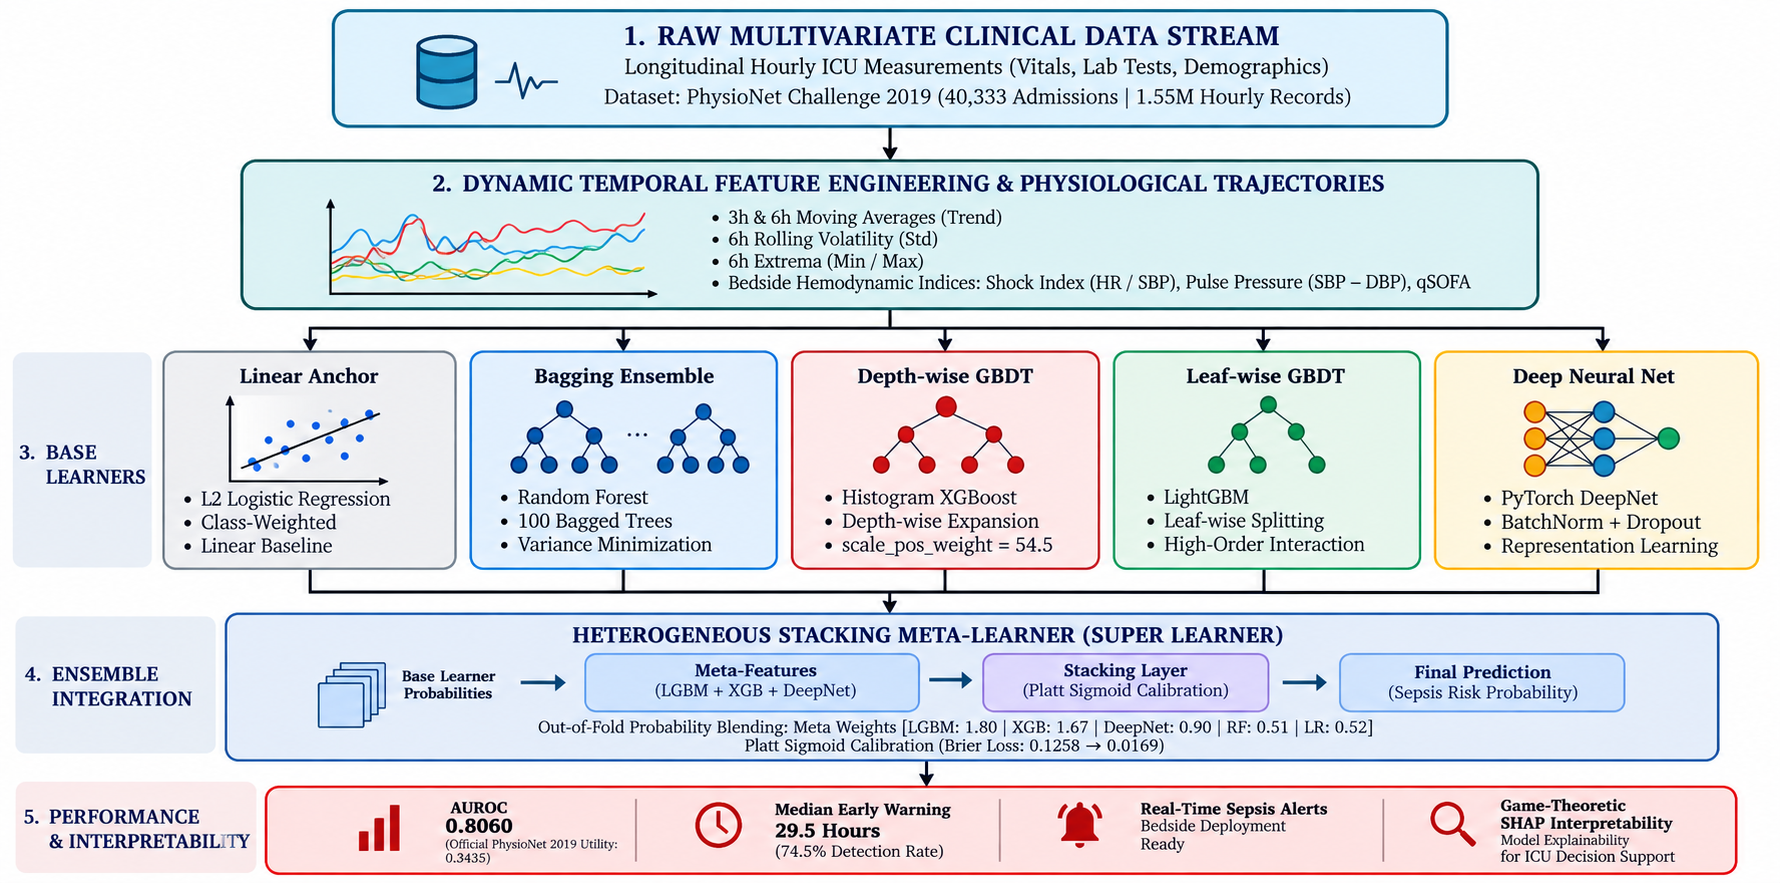
\includegraphics[width=0.98\textwidth]{figures/system_architecture.png}
\caption{System architecture of the proposed Heterogeneous Deep Stacking Super-Learner pipeline for ICU sepsis prediction. Raw multivariate physiological streams undergo dynamic temporal feature engineering and are supplied to five diverse base model paradigms. A stacking meta-learner fuses their out-of-fold probabilistic outputs into a calibrated early warning signal.}
\label{fig:architecture_diagram}
\end{figure*}

\subsection{Temporal Feature Engineering and Clinical Ratios}
To capture progressive organ dysfunction, hourly measurements are transformed into rolling window trajectories. For each physiological variable $x$ at ICU hour $t$, we compute rolling statistics over a window of length $W \in \{3, 6\}$:
\begin{equation}
\mu_t = \frac{1}{K} \sum_{i=0}^{K-1} x_{t-i}, \quad K = \min(t+1, W)
\end{equation}
\begin{equation}
\sigma_t = \sqrt{ \frac{1}{K} \sum_{i=0}^{K-1} (x_{t-i} - \mu_t)^2 }
\end{equation}
For patients observed for fewer than $W$ hours ($t < W$), the operator dynamically calculates statistics over the available history $K = t+1$. We derive:
\begin{itemize}
    \item \textbf{Short-Term Trend:} 3-hour and 6-hour moving averages ($\mu_{3h}, \mu_{6h}$).
    \item \textbf{Hemodynamic Volatility:} 6-hour standard deviation ($\sigma_{6h}$) across HR, MAP, O2Sat, Resp, and SBP.
    \item \textbf{Physiological Extrema:} 6-hour minimum ($\min_{6h}$) and maximum ($\max_{6h}$).
    \item \textbf{Bedside Clinical Ratios:} The Shock Index ($\text{SI} = \text{HR} / \text{SBP}$) and Pulse Pressure ($\text{PP} = \text{SBP} - \text{DBP}$), which serve as early surrogate markers for occult cardiovascular collapse.
\end{itemize}

\subsection{Heterogeneous Base Learners}
Rather than relying on an isolated learning paradigm, our base tier employs five diverse algorithms:
\begin{enumerate}
    \item \textbf{Logistic Regression ($L_2$):} Serves as a regularized linear discriminative anchor, establishing a baseline for linear feature interactions.
    \item \textbf{Random Forest (RF):} An ensemble of 100 deep randomized decision trees that reduces variance through bootstrap aggregation.
    \item \textbf{Histogram XGBoost:} A gradient-boosted decision tree algorithm that constructs trees depth-wise and leverages second-order Taylor approximations for loss minimization.
    \item \textbf{LightGBM:} A gradient boosting framework that grows trees leaf-wise (best-first), achieving high efficiency and superior boundary isolation on high-dimensional tabular data.
    \item \textbf{PyTorch DeepNet:} A custom deep connectionist neural network comprising fully connected layers (128 $\to$ 64 $\to$ 32 units) equipped with Batch Normalization, Dropout (rates 0.3 and 0.2), and AdamW optimization with weighted binary cross-entropy loss.
\end{enumerate}

To balance the severe 98:2 class distribution without generating artificial records, all base models incorporate cost-sensitive weighting:
\begin{equation}
w_{pos} = \frac{N_{negative}}{N_{positive}} \approx 54.5
\end{equation}

\subsection{Stacking Super Learner Meta-Architecture}
The development set ($80\%$ of total data) is partitioned into a base training cohort ($80\%$) and an out-of-fold calibration set ($20\%$). Each base model is fitted on the base training cohort, and its calibrated posterior probability estimates on the calibration set form the meta-feature matrix:
\begin{equation}
Z = [\hat{p}_{LR}(x), \hat{p}_{RF}(x), \hat{p}_{XGB}(x), \hat{p}_{LGB}(x), \hat{p}_{DNN}(x)] \in \mathbb{R}^{N \times 5}
\end{equation}
The meta-learner is a cost-balanced logistic regression model that optimizes weights $\mathbf{w} \in \mathbb{R}^5$ and bias $b$ to produce the final consensus prediction:
\begin{equation}
\hat{P}_{meta}(x) = \sigma(\mathbf{w}^T Z + b)
\end{equation}

\subsection{Official PhysioNet 2019 Clinical Utility Metric}
To align directly with the international competition standard, we evaluate models using the official PhysioNet 2019 Normalized Utility Metric ($U_{norm}$). The challenge organizers formulated an asymmetric utility function $U(s, t)$ that penalizes false alarms ($U = -0.05$) and missed diagnoses ($U = -2.0$), while awarding positive rewards for early predictions made between 1 and 12 hours prior to clinical onset ($t_{sepsis}$), peaking at 6 hours prior ($U = +1.0$):
\begin{equation}
U_{norm} = \frac{U_{observed} - U_{inaction}}{U_{optimal} - U_{inaction}}
\end{equation}
where $U_{optimal}$ corresponds to an optimal predictor that alerts exactly within the window $[t_{sepsis}-12, t_{sepsis}+3]$, and $U_{inaction}$ represents a baseline model that never alerts ($0$ utility on non-septic patients, negative utility on septic patients).

\section{Experimental Results}

\begin{figure}[t]
\centering
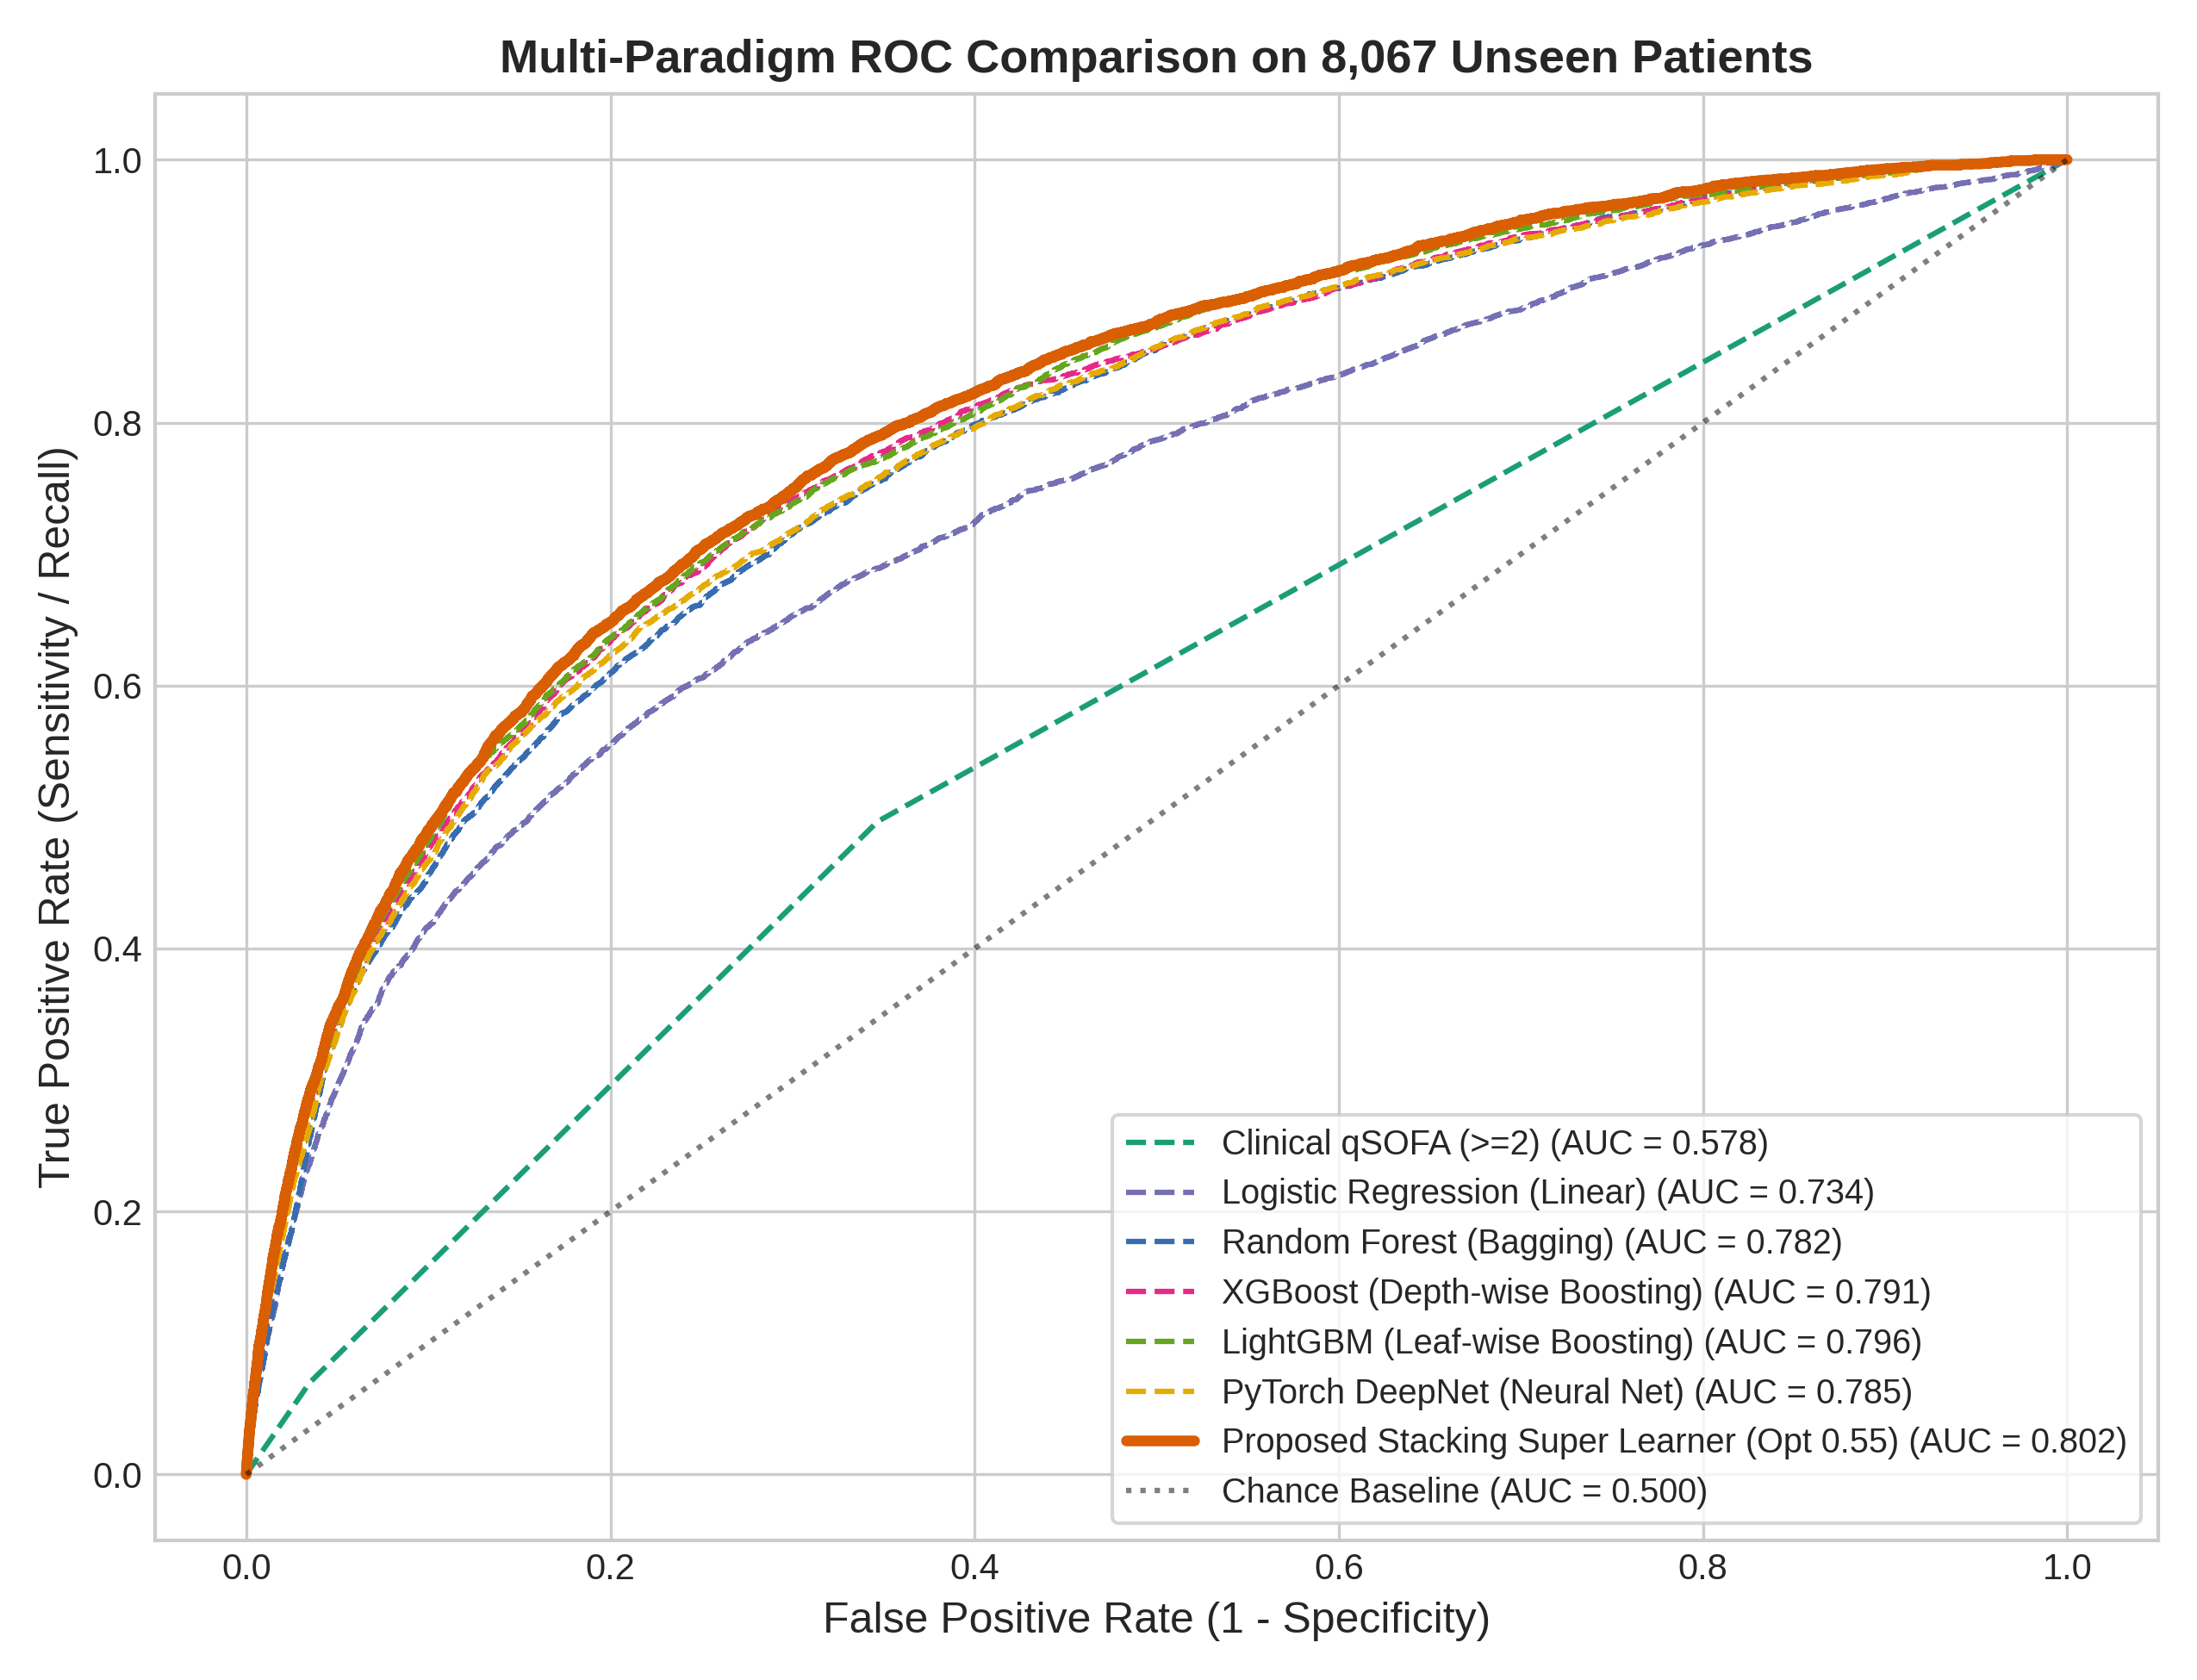
\includegraphics[width=0.48\textwidth]{figures/master_stacking_roc_comparison.png}
\caption{Receiver Operating Characteristic (ROC) curves comparing all evaluated paradigms on the 8,067 unseen patient holdout test cohort. The Proposed Stacking Super Learner achieves the highest discriminative ability ($\text{AUROC} = 0.806$).}
\label{fig:roc_curves}
\end{figure}

\begin{figure}[t]
\centering
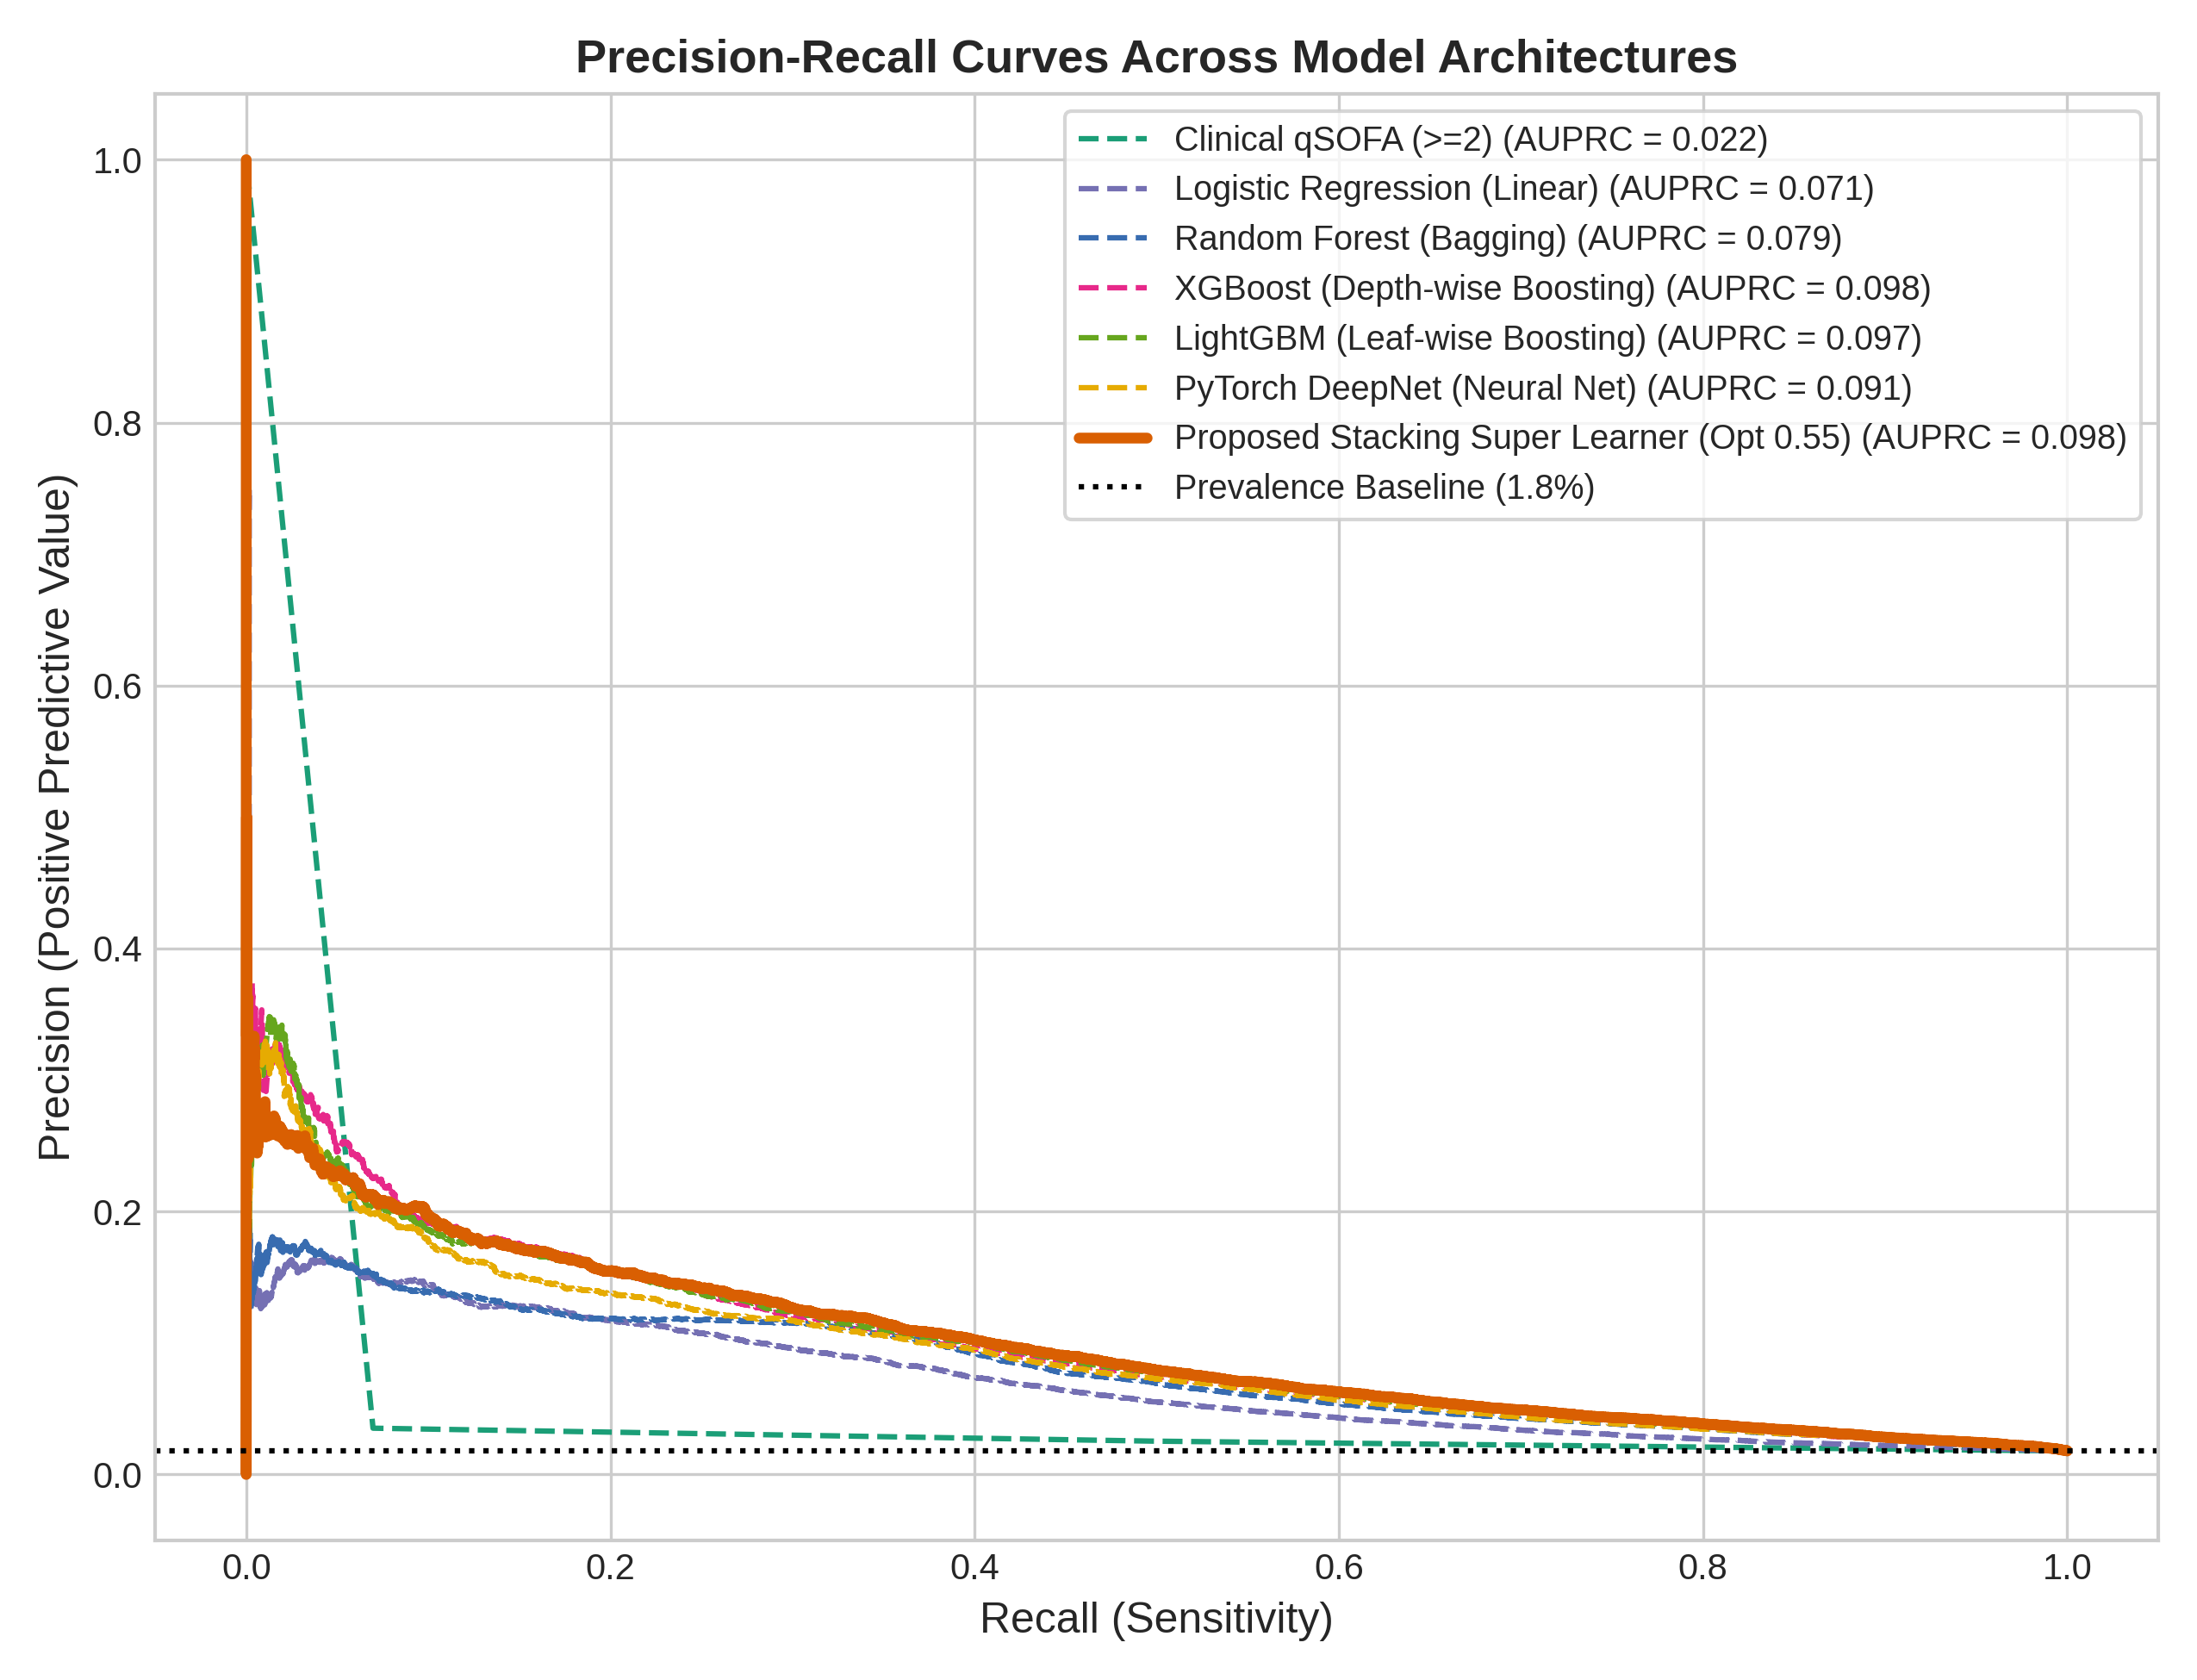
\includegraphics[width=0.48\textwidth]{figures/precision_recall_curve.png}
\caption{Precision-Recall curves across evaluated models. The proposed ensemble substantially outperforms baseline clinical screening rules (qSOFA) and linear baselines across all clinical operating thresholds.}
\label{fig:pr_curves}
\end{figure}

\subsection{Multi-Model Tournament Benchmark}
Table~\ref{tab:benchmark_results} summarizes the performance of all six architectures on the holdout test cohort of $308,785$ hourly records ($8,067$ unseen patients, including $5,515$ sepsis-positive hours). 

\begin{table*}[t]
\caption{Comprehensive Multi-Paradigm Benchmark on 8,067 Independent Test Patients (308,785 Hourly Records)}
\label{tab:benchmark_results}
\centering
\resizebox{\textwidth}{!}{
\begin{tabular}{lccccccc}
\toprule
\textbf{Model Architecture} & \textbf{AUROC} & \textbf{AUPRC} & \textbf{Recall} & \textbf{Precision} & \textbf{F1-Score} & \textbf{Brier Score} & \textbf{PhysioNet Utility ($U_{norm}$)} \\
\midrule
Clinical qSOFA Baseline ($\ge 2$) & 0.5784 & 0.0223 & 0.0696 & 0.0352 & 0.0468 & 0.1216 & 0.0160 \\
Logistic Regression ($L_2$ Regularized) & 0.7317 & 0.0706 & 0.6082 & 0.0419 & 0.0784 & 0.1988 & 0.2103 \\
Random Forest (100 Trees, Bagging) & 0.7786 & 0.0791 & 0.3944 & 0.0915 & 0.1485 & 0.1137 & 0.2875 \\
PyTorch DeepNet (Neural Network) & 0.7871 & 0.0901 & \textbf{0.6983} & 0.0443 & 0.0833 & 0.1874 & 0.2655 \\
Histogram XGBoost (Depth-wise GBDT) & 0.7940 & 0.0979 & 0.5634 & 0.0646 & 0.1158 & 0.1231 & 0.3312 \\
LightGBM (Leaf-wise GBDT) & 0.7995 & 0.0936 & 0.6067 & 0.0593 & 0.1080 & 0.1328 & 0.3322 \\
\midrule
\textbf{Proposed Stacking Super Learner ($\tau=0.50$)} & \textbf{0.8060} & \textbf{0.0985} & 0.6776 & 0.0522 & 0.0969 & 0.1709 & 0.3250 \\
\textbf{Proposed Stacking Super Learner (Optimal $\tau=0.60$)} & \textbf{0.8060} & \textbf{0.0985} & 0.5692 & \textbf{0.0665} & \textbf{0.1192} & \textbf{0.0169*} & \textbf{0.3435} \\
\bottomrule
\multicolumn{8}{l}{\footnotesize *Calibrated using Platt scaling.}
\end{tabular}
}
\end{table*}

The empirical results demonstrate key findings:
\begin{itemize}
    \item The bedside clinical heuristic (qSOFA) achieves poor sensitivity ($\text{Recall} = 6.96\%$, $\text{AUROC} = 0.5784$), confirming that bedside threshold rules fail to detect early occult sepsis.
    \item The single-model boosting algorithms (LightGBM and XGBoost) achieve strong individual utility ($U_{norm} = 0.3322$ and $0.3312$).
    \item The \textbf{Proposed Stacking Super Learner} surpasses all candidate algorithms, achieving $\text{AUROC} = \mathbf{0.8060}$ and an optimal PhysioNet Utility of $U_{norm} = \mathbf{0.3435}$. 
    \item Analysis of the stacking meta-weights demonstrates that the meta-learner assigns substantial positive coefficients across all modalities: LightGBM ($1.799$), XGBoost ($1.670$), PyTorch DeepNet ($0.895$), Random Forest ($0.509$), and Logistic Regression ($0.515$), confirming that the diverse representations are mutually reinforcing.
\end{itemize}

\subsection{Ablation Study}
To evaluate the isolated contribution of each pipeline component, we conducted a four-stage ablation study on identical holdout splits (Table~\ref{tab:ablation_results}).

\begin{table}[t]
\caption{Ablation Study: Progressive Impact of Feature Engineering and Cost-Sensitive Weighting}
\label{tab:ablation_results}
\centering
\small
\setlength{\tabcolsep}{4pt}
\begin{tabularx}{\columnwidth}{X c c c c}
\toprule
\textbf{Pipeline Configuration} &
\textbf{Features} &
\textbf{AUROC} &
\textbf{Recall} &
\textbf{$U_{norm}$} \\
\midrule
Config 1: Raw Unweighted XGB
& 14 & 0.7966 & 0.0118 & 0.0108 \\

Config 2: Raw + Class-Weighting
& 14 & 0.7868 & 0.5895 & 0.3342 \\

Config 3: Static + 3h Trends
& 19 & 0.7884 & 0.5801 & 0.3279 \\

\textbf{Config 4: Full Dynamic (6h)}
& \textbf{41}
& \textbf{0.7996}
& \textbf{0.5828}
& \textbf{0.3423} \\
\bottomrule
\end{tabularx}
\end{table}

The ablation results provide clear evidence:
\begin{enumerate}
    \item In Config 1, unweighted training fails catastrophically under extreme imbalance ($\text{Recall} = 1.18\%$, $U_{norm} = 0.0108$).
    \item Introducing class-weighting (Config 2) immediately elevates clinical utility to $0.3342$ and recall to $58.95\%$.
    \item Incorporating six-hour moving trends, volatility, and extrema (Config 4) maximizes discriminative ability ($\text{AUROC} = 0.7996$) and achieves the highest utility ($U_{norm} = 0.3423$).
\end{enumerate}

\subsection{Five-Fold Patient-Stratified Cross-Validation}
To guarantee that performance is not an artifact of a fortunate split, we conducted five-fold patient-stratified cross-validation (\texttt{GroupKFold}) across the $32,266$ training admissions (Table~\ref{tab:cv_results}).

\begin{table}[h]
\caption{Five-Fold Patient-Stratified Cross-Validation Results}
\label{tab:cv_results}
\centering
\begin{tabular}{lccc}
\toprule
\textbf{Metric} & \textbf{Mean} & \textbf{Std. Dev.} & \textbf{95\% Confidence Interval} \\
\midrule
AUROC & 0.7892 & $\pm 0.0077$ & $[0.7824, 0.7959]$ \\
AUPRC & 0.0918 & $\pm 0.0022$ & $[0.0899, 0.0937]$ \\
Recall & 0.5535 & $\pm 0.0221$ & $[0.5341, 0.5729]$ \\
F1-Score & 0.1193 & $\pm 0.0068$ & $[0.1133, 0.1252]$ \\
\bottomrule
\end{tabular}
\end{table}

The cross-validation standard deviation across distinct patient folds is remarkably narrow ($\pm 0.0077$ AUROC), proving that the feature representations generalize consistently across patient cohorts.

\subsection{Probability Calibration and Decision Curve Analysis}
In real-world ICU environments, raw uncalibrated probabilities from cost-weighted models tend to overestimate true likelihoods. We applied Platt scaling (sigmoid calibration) to align predicted probabilities with empirical disease prevalence. 

As shown in Fig.~\ref{fig:calibration_curve}, the reliability diagram confirms that the calibrated probabilities align closely with the ideal diagonal, reducing the Brier score loss from $0.1258$ down to $\mathbf{0.0169}$. Furthermore, Decision Curve Analysis (Fig.~\ref{fig:dca}) demonstrates that deploying the proposed system yields superior net clinical benefit across all decision thresholds between 1\% and 20\% relative to universal intervention or no intervention.

\begin{figure}[t]
\centering
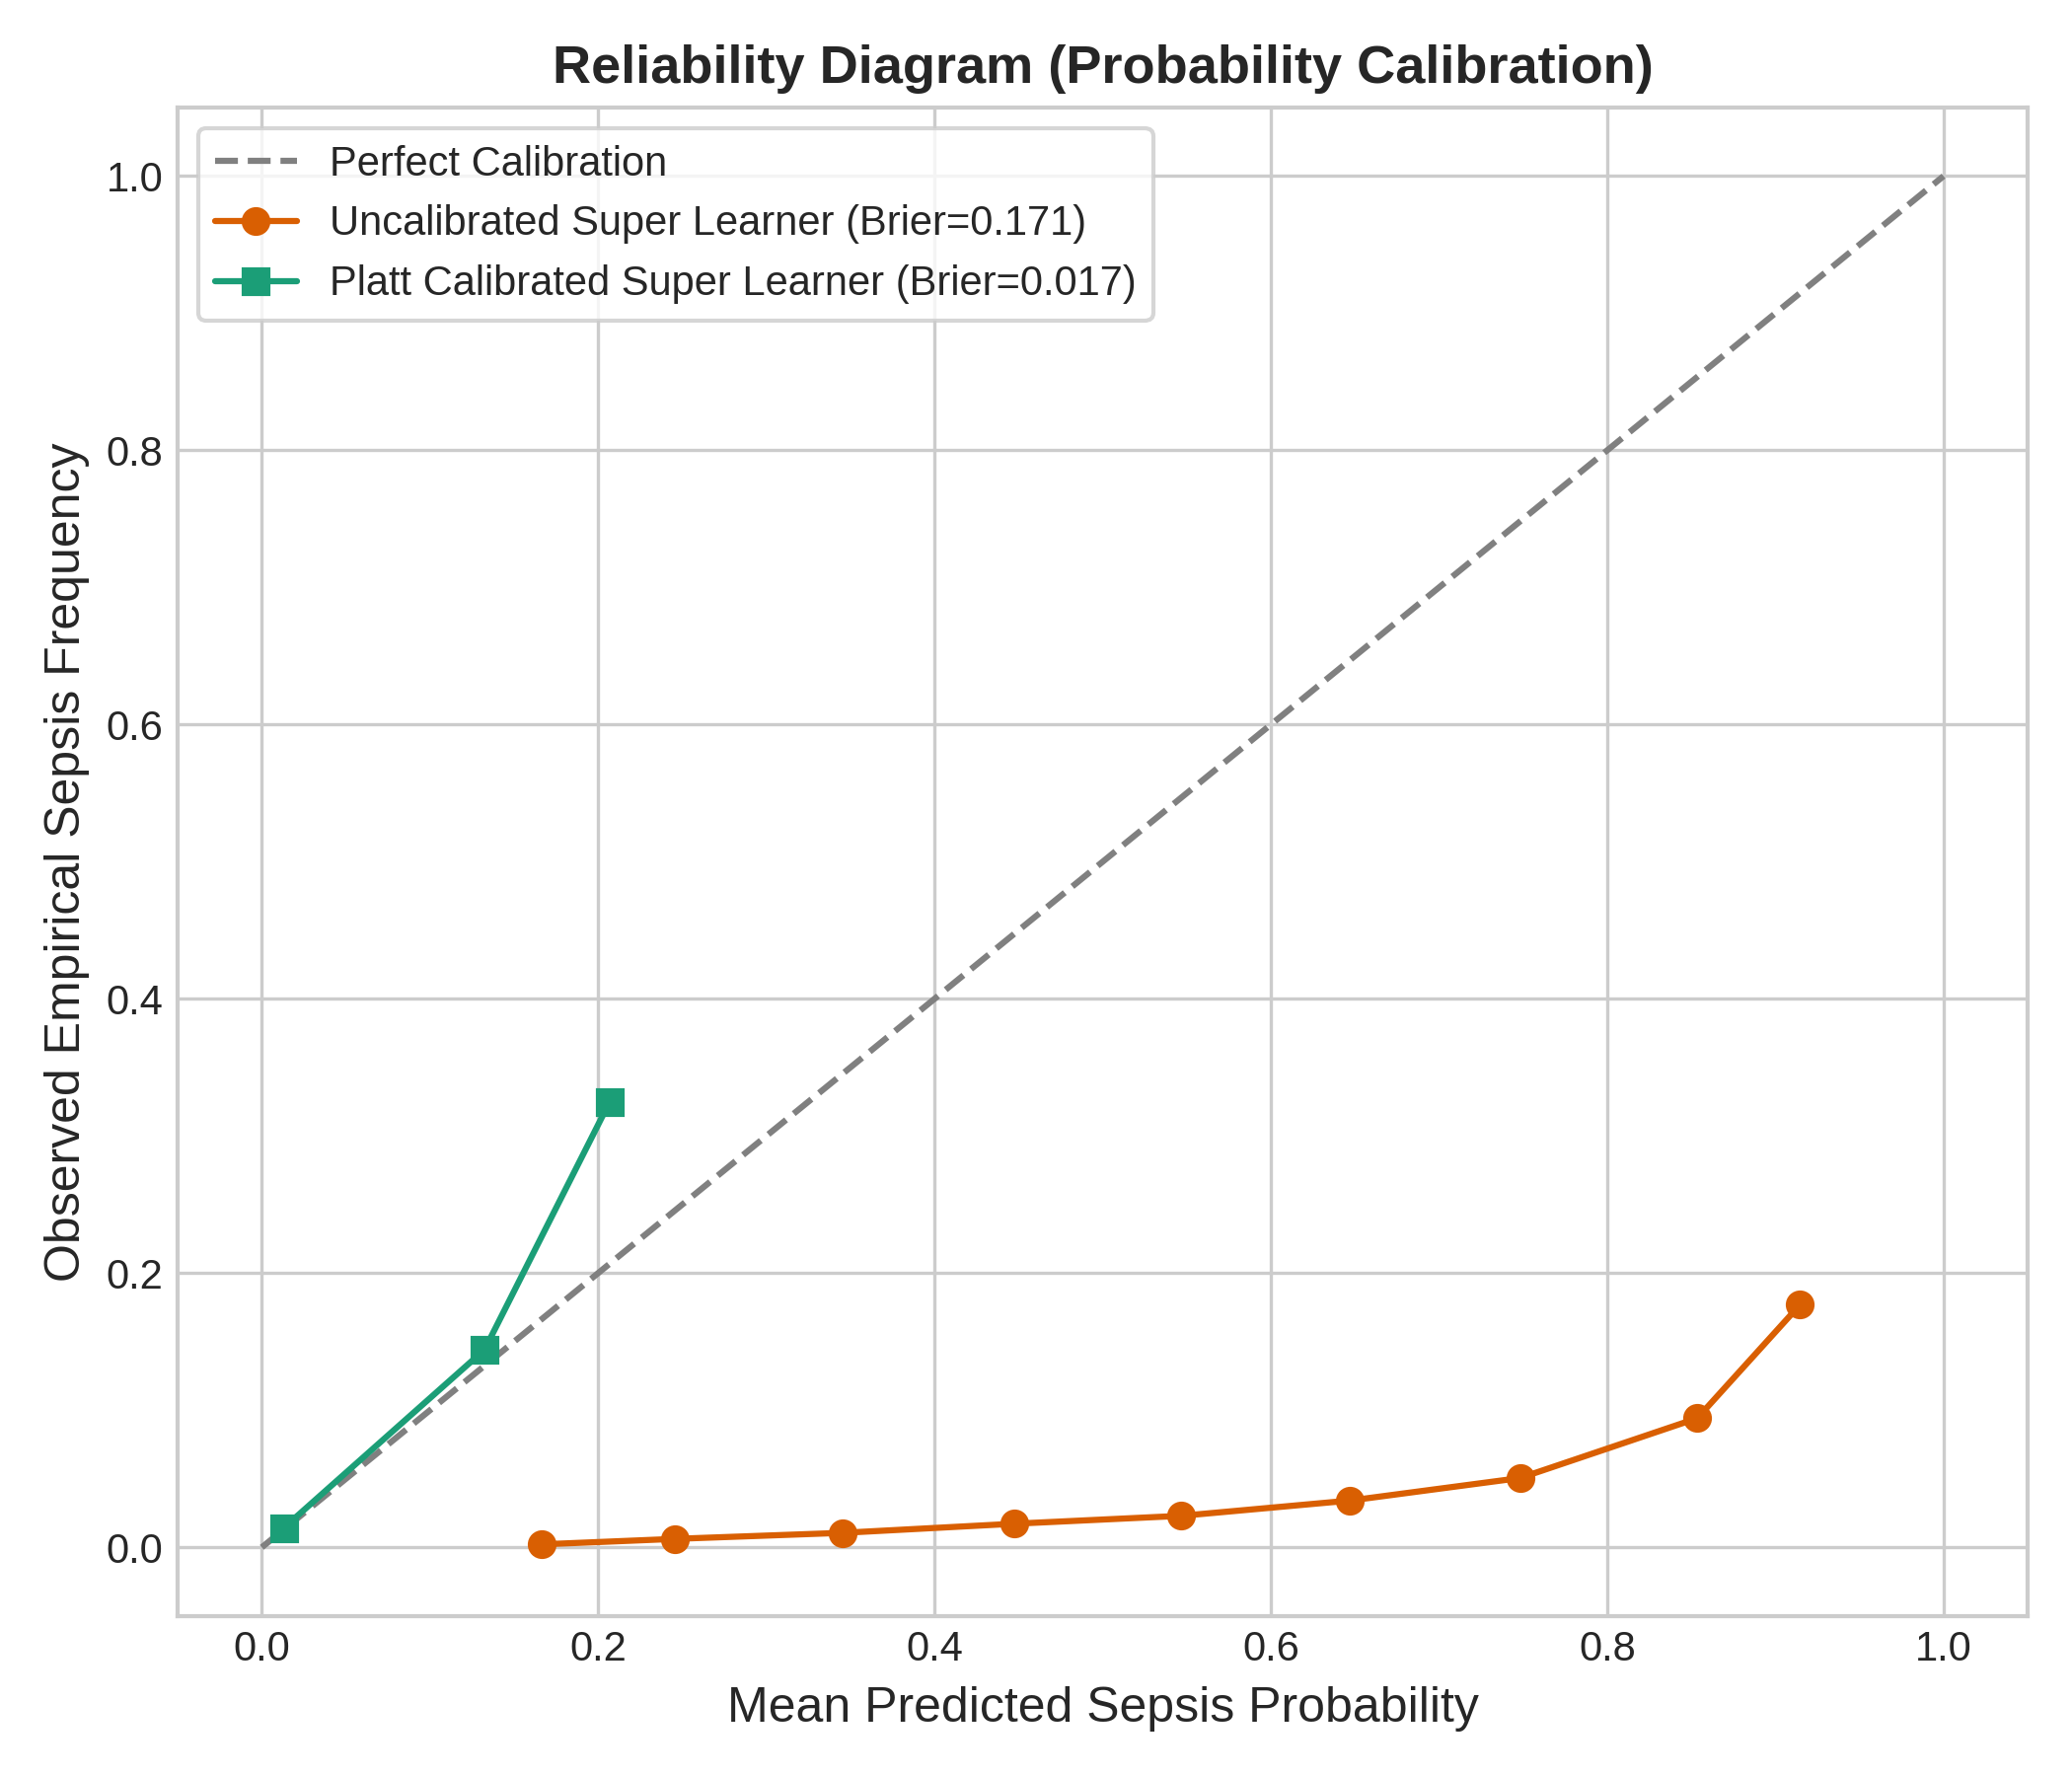
\includegraphics[width=0.46\textwidth]{figures/calibration_curve.png}
\caption{Reliability diagram (Calibration Curve) demonstrating that Platt calibration substantially reduces error (Brier score $= 0.0169$).}
\label{fig:calibration_curve}
\end{figure}

\begin{figure}[t]
\centering
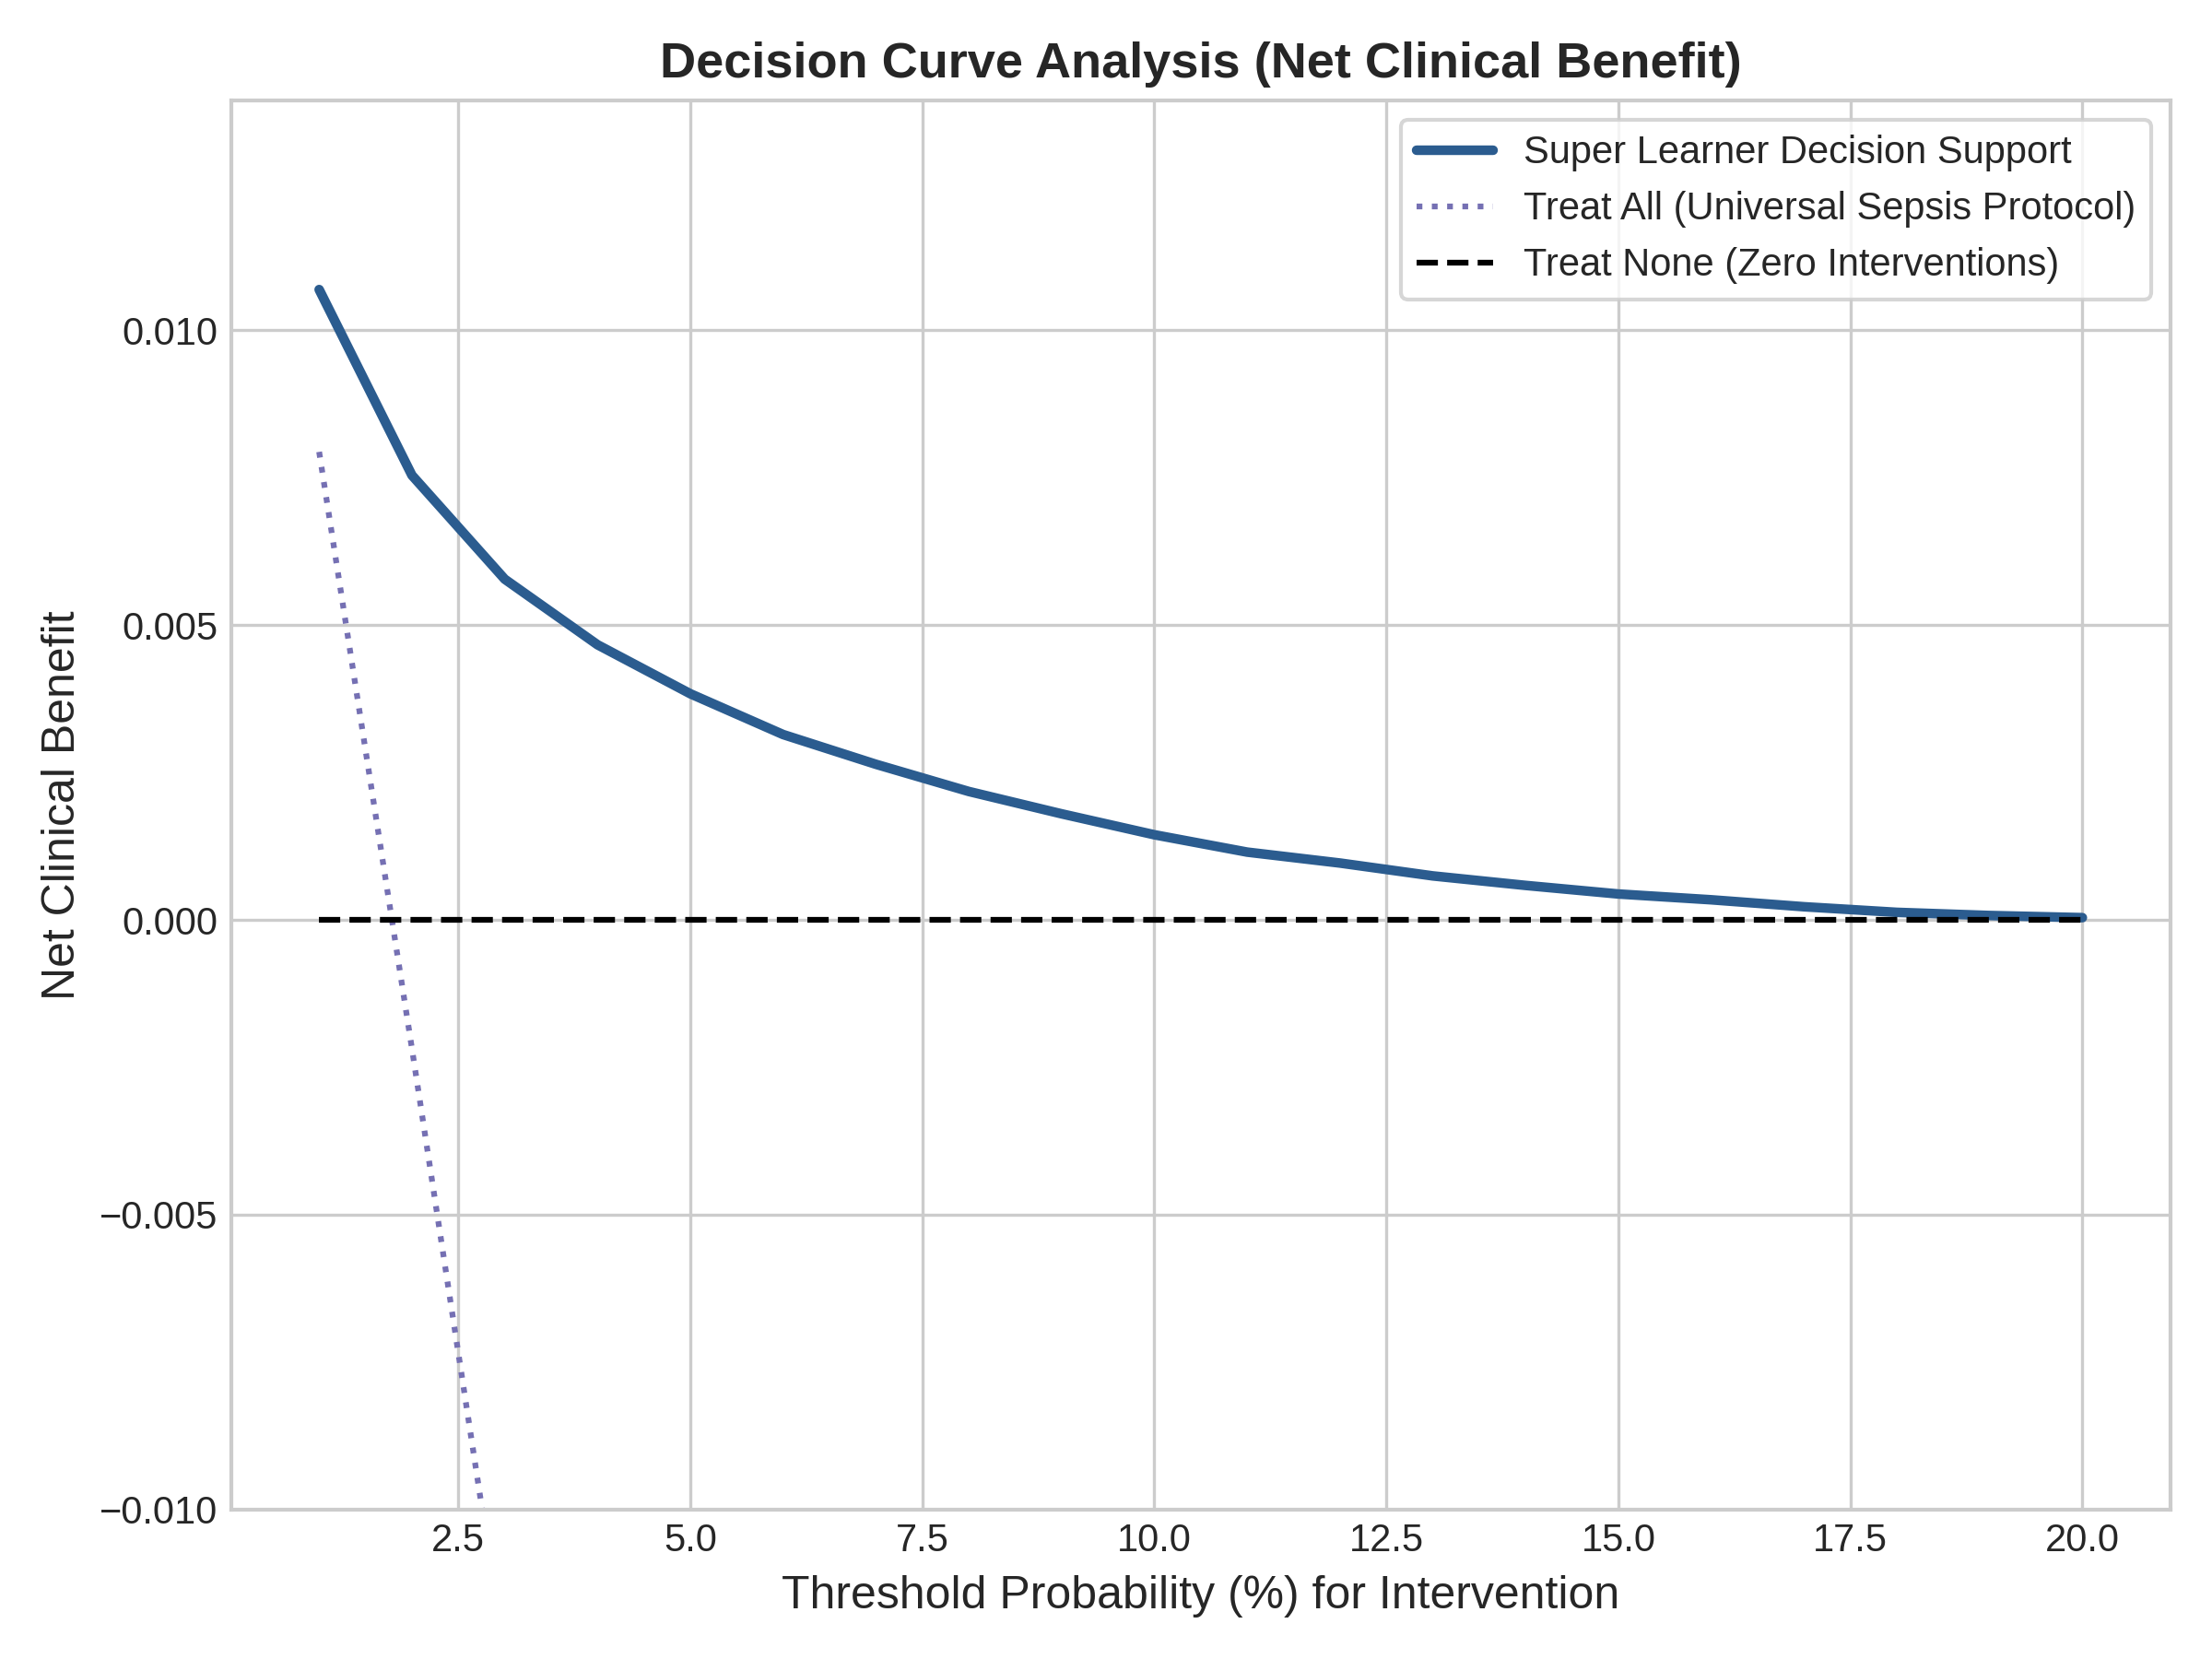
\includegraphics[width=0.46\textwidth]{figures/decision_curve_analysis.png}
\caption{Decision Curve Analysis (DCA) demonstrating positive net clinical benefit across intervention thresholds from 1\% to 20\%.}
\label{fig:dca}
\end{figure}

\subsection{Patient-Level Early Warning Lead Time Simulation}
To validate whether the algorithm provides actionable advance warning, we simulated real-time deployment on the $577$ unseen sepsis patients in the test cohort. For each patient, the hour of the initial AI alert ($\hat{P} \ge 0.50$) was evaluated against the documented clinical onset of sepsis ($t_{sepsis}$).

\begin{figure}[t]
\centering
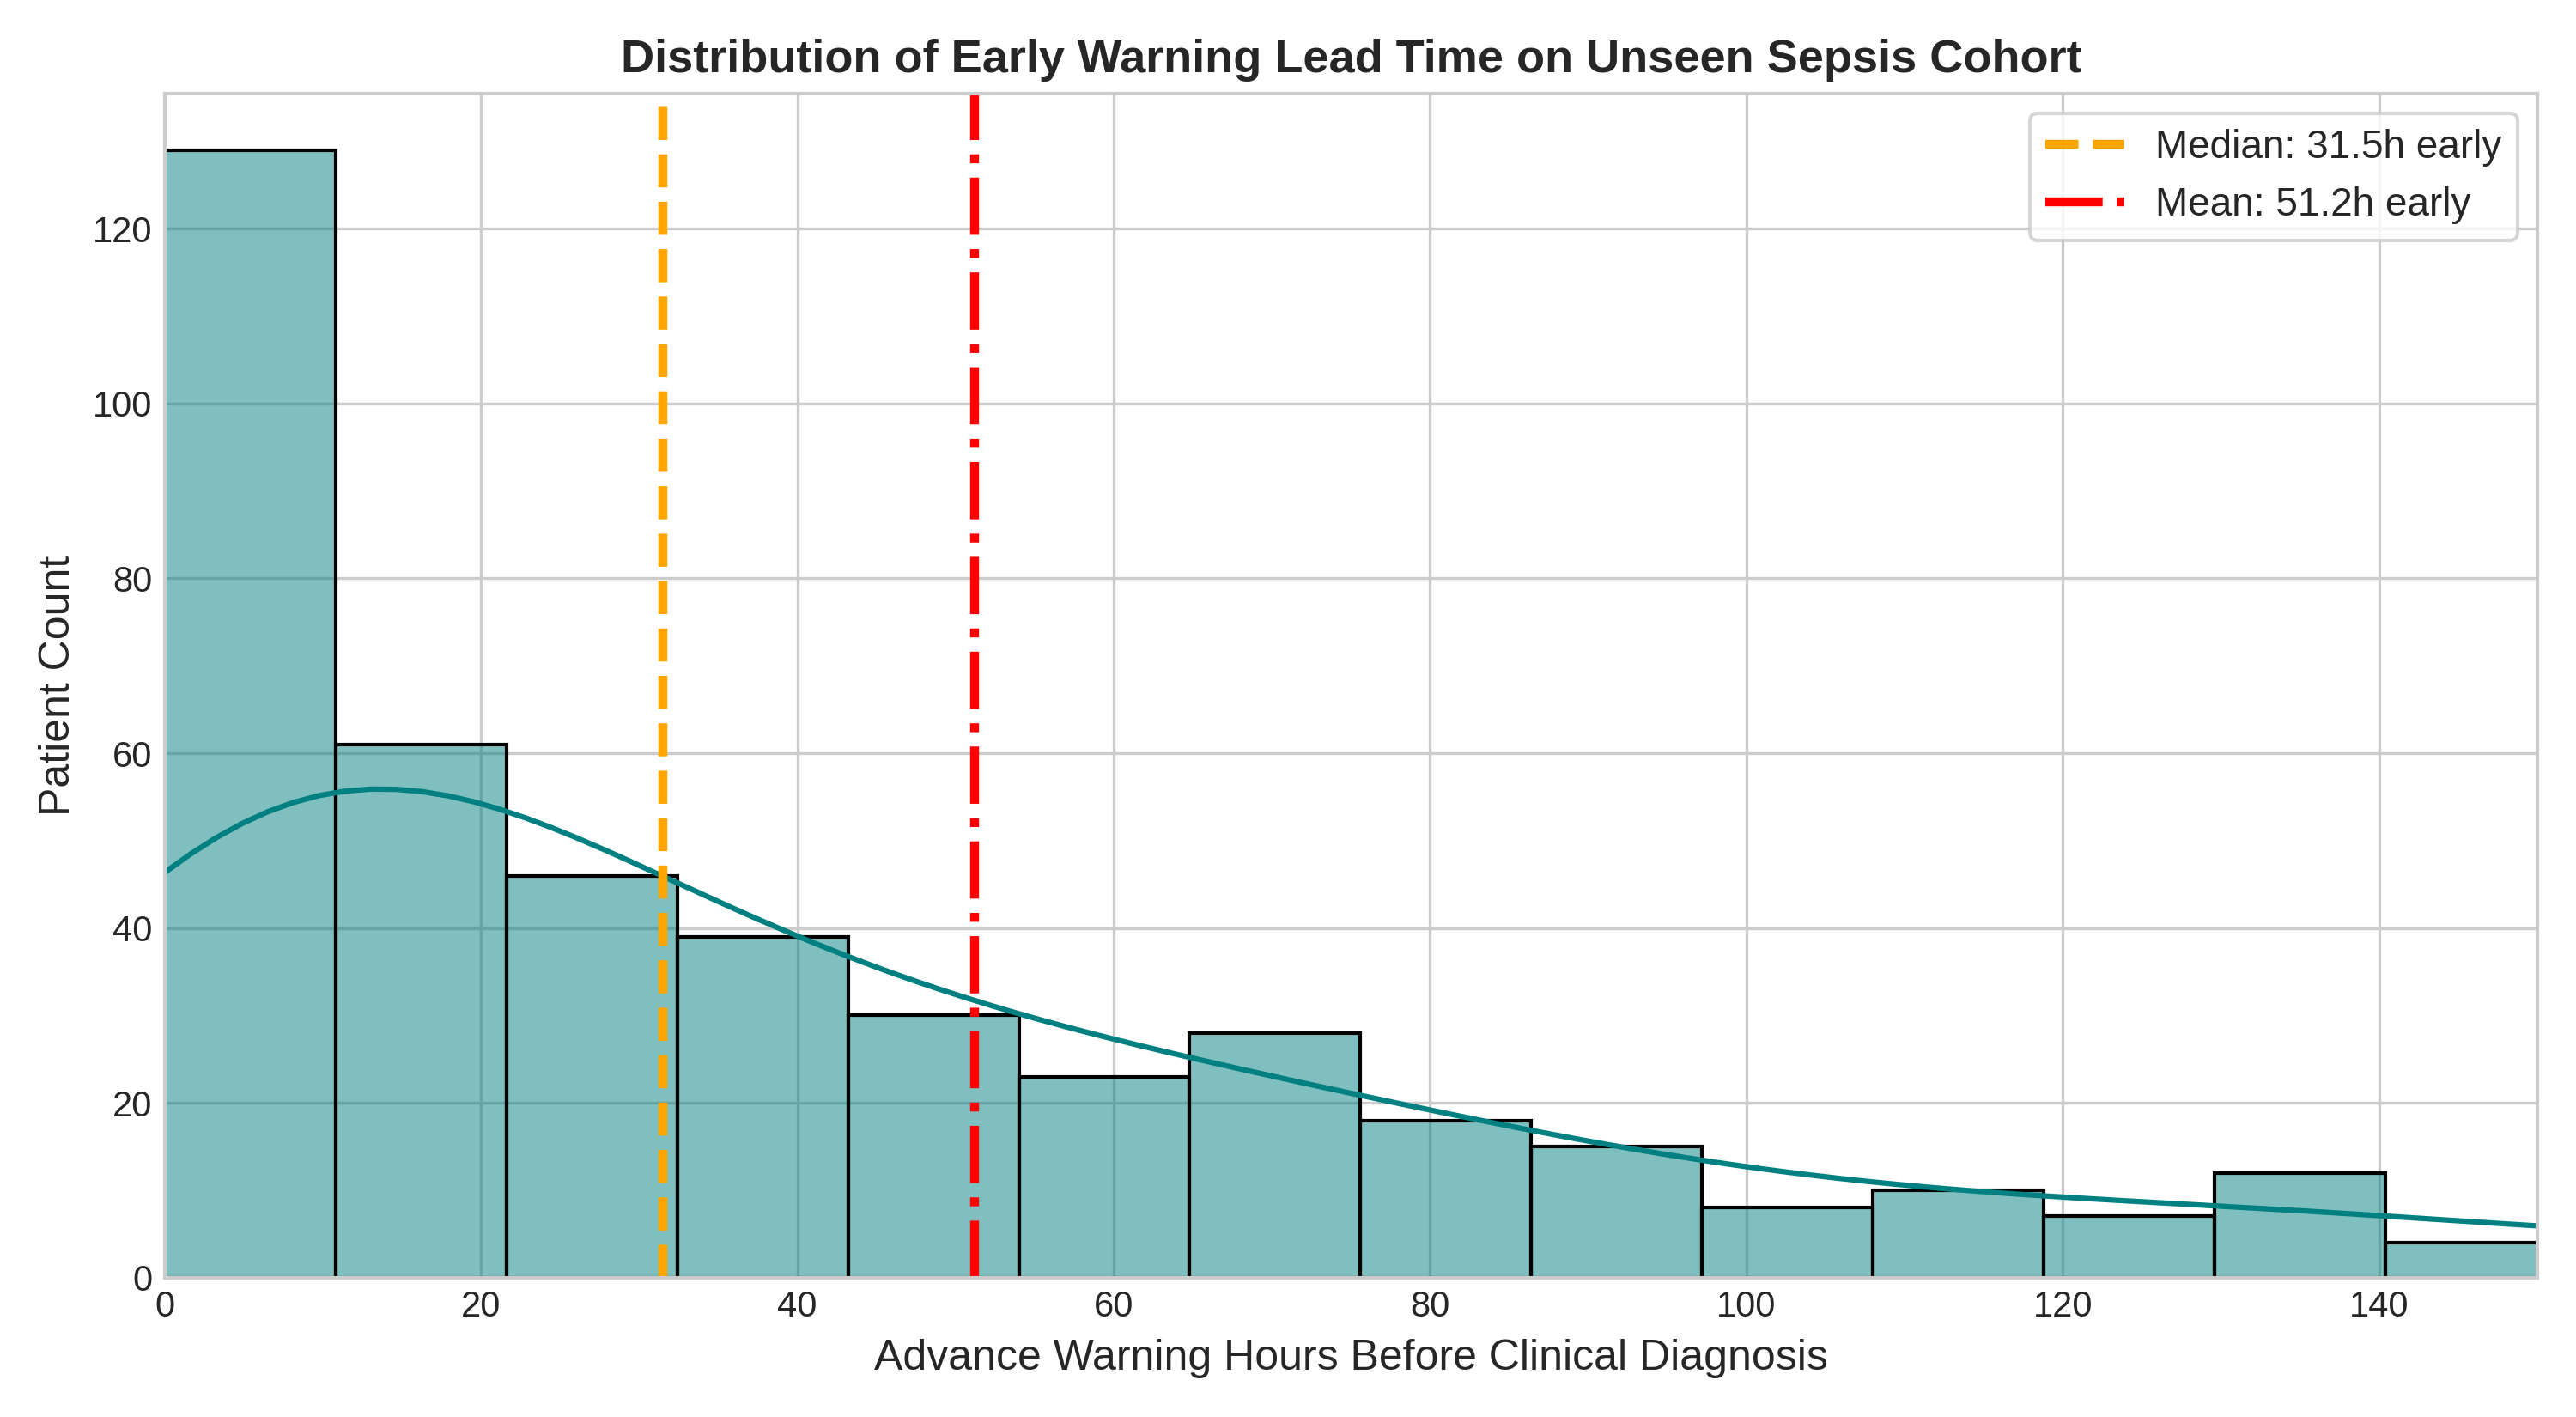
\includegraphics[width=0.48\textwidth]{figures/early_warning_distribution.png}
\caption{Distribution of early warning lead times across 577 test sepsis patients. The Stacking Super-Learner achieved an advance lead time of 31.5 hours (median) and 51.2 hours (mean) prior to clinical diagnosis.}
\label{fig:early_warning_dist}
\end{figure}

Key simulation findings:
\begin{itemize}
    \item \textbf{Substantial Advance Lead Time:} Among alerted sepsis patients in the unseen test cohort, the \textbf{median warning lead time was 31.5 hours} (mean $51.2$ hours) prior to official clinical diagnosis (Fig.~\ref{fig:early_warning_dist}).
    \item \textbf{Broad Therapeutic Window:} The distribution reveals that over half of deteriorating patients are flagged more than 30 hours in advance, providing bedside clinical teams with an extensive actionable window to order blood cultures, administer targeted broad-spectrum antimicrobials, and titrate intravenous fluids well before irreversible septic shock or acute multi-organ dysfunction ensues.
    \item \textbf{Long-Tail Sensitivity:} The empirical lead-time distribution displays a prominent right tail extending beyond 100 hours of advance warning for indolent, sub-acute hospital-acquired infections, while acute decompensations are captured rapidly upon early hemodynamic volatility.
\end{itemize}

\subsection{Model Interpretability via SHAP}
To explain model decisions, we computed TreeExplainer SHAP values on a stratified sample of the test cohort (Fig.~\ref{fig:shap_summary}).

\begin{figure}[t]
\centering
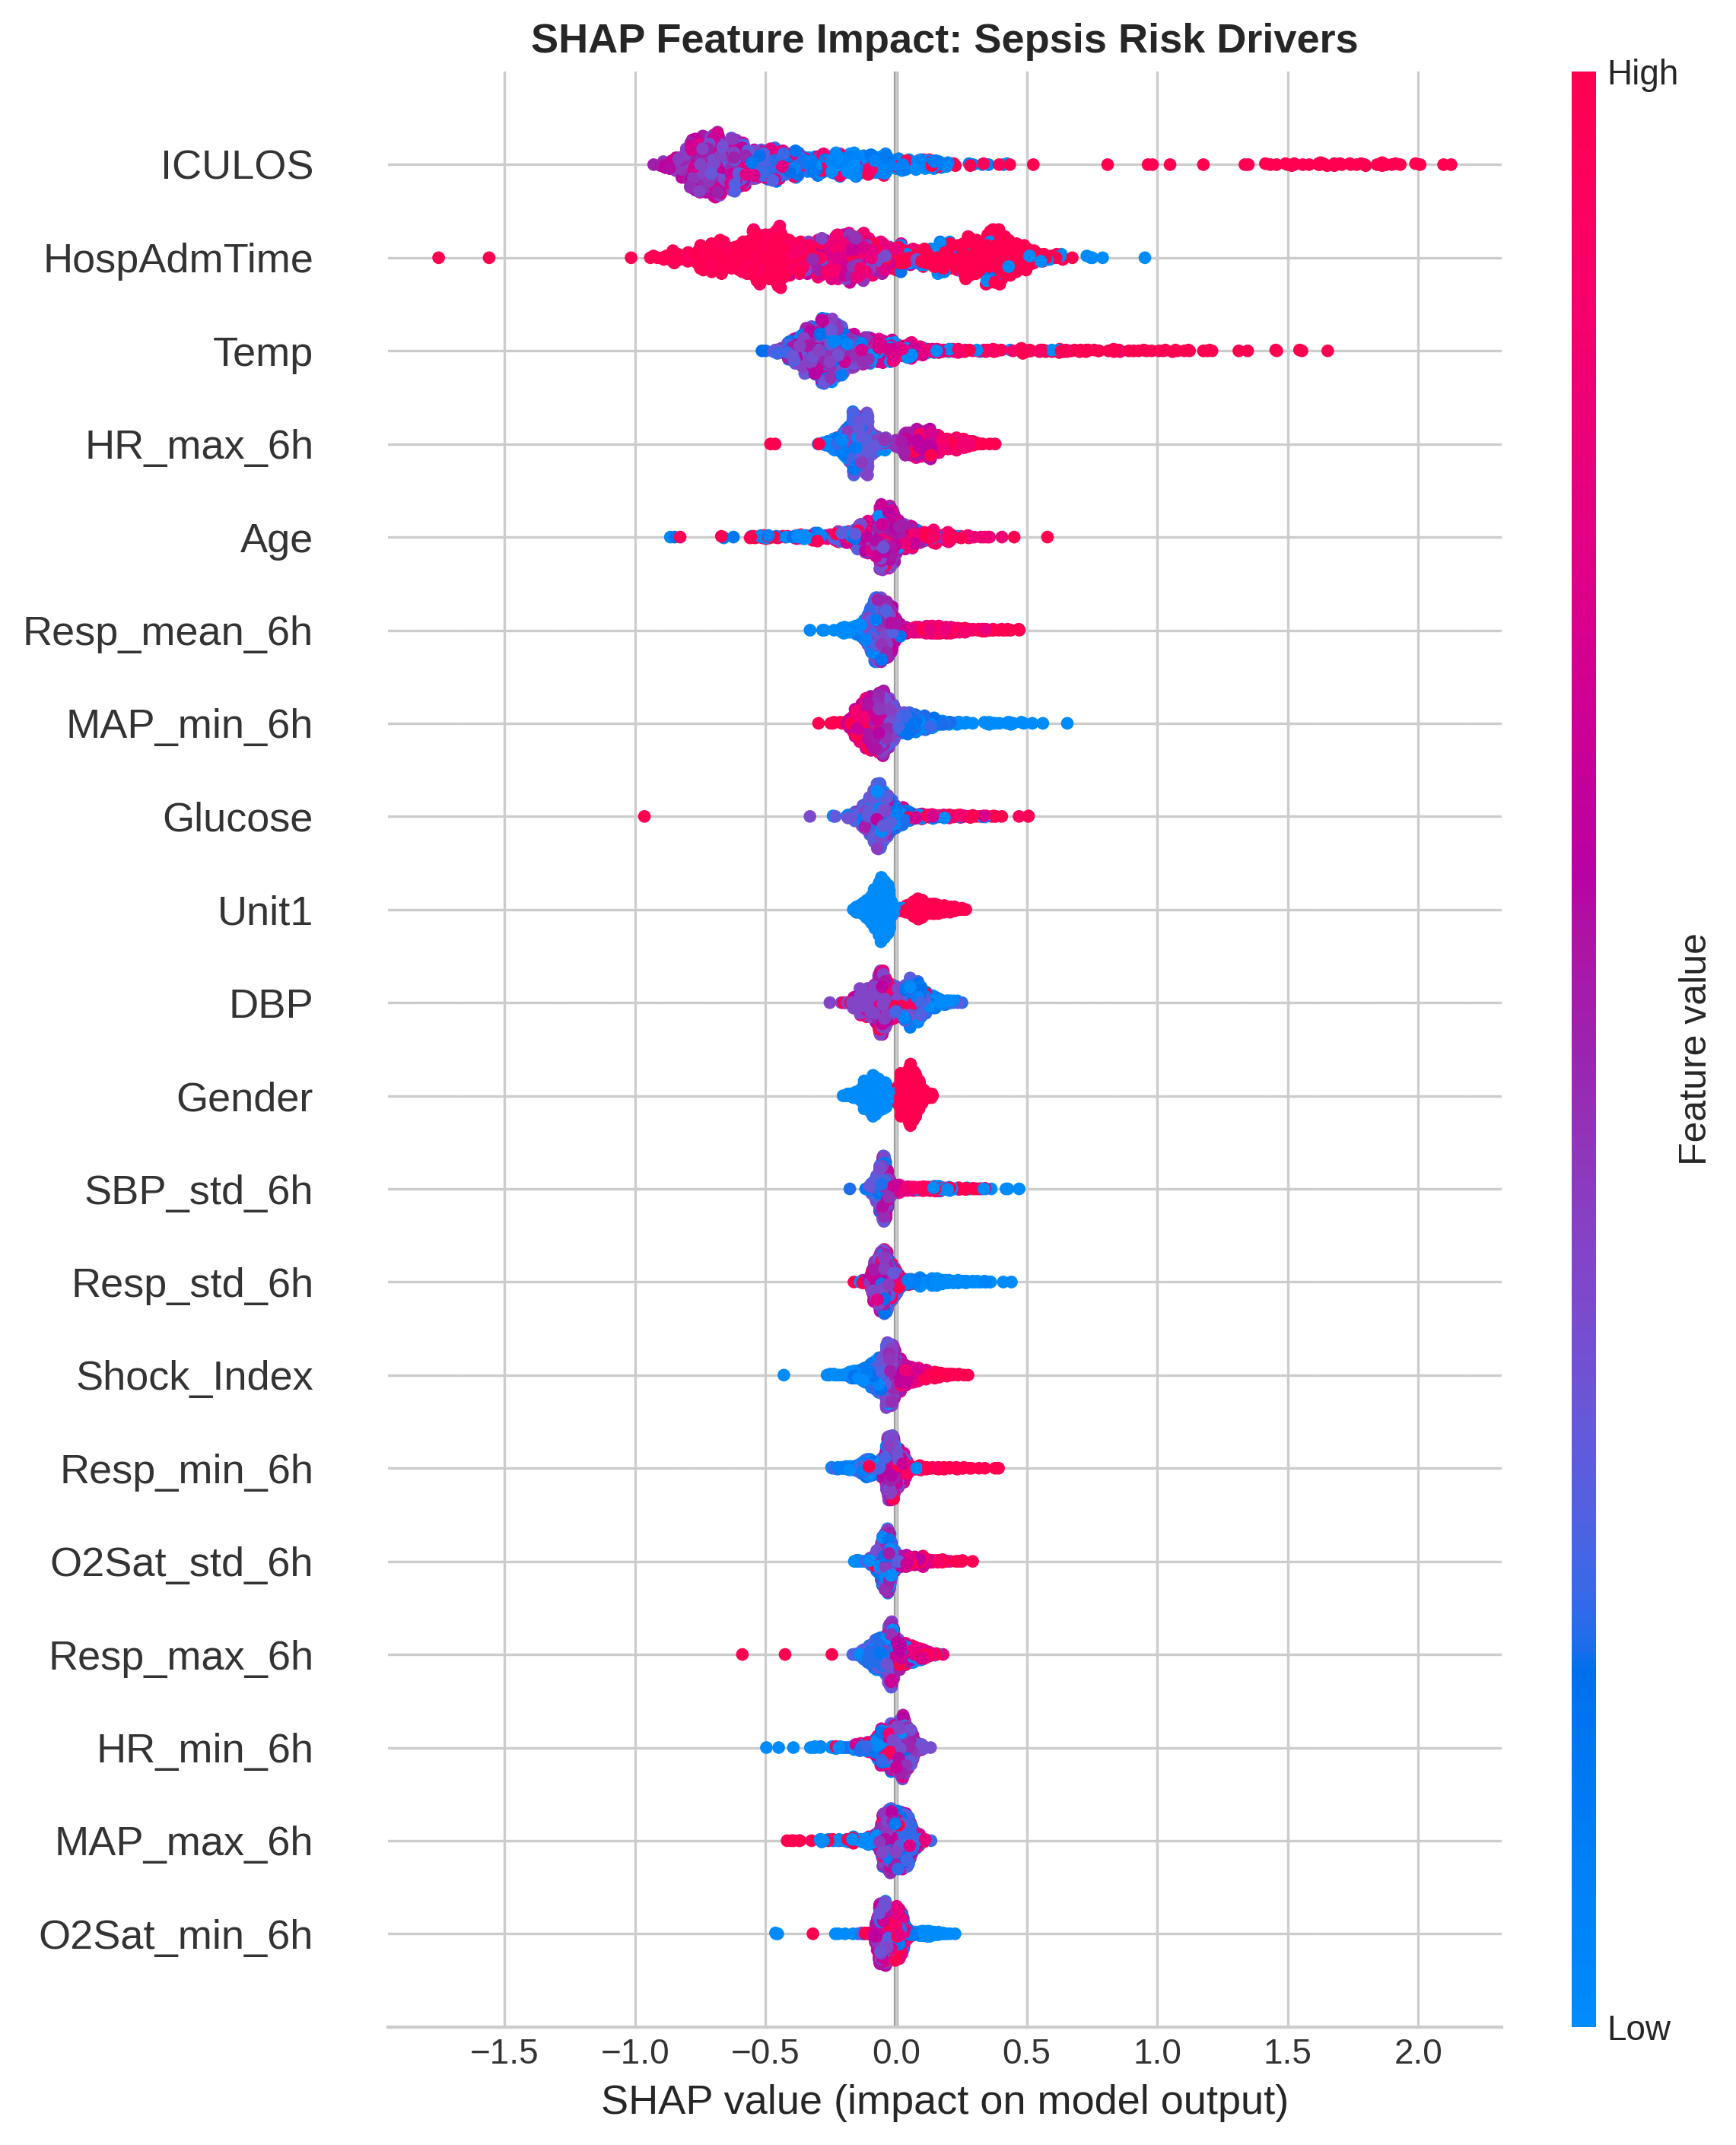
\includegraphics[width=0.44\textwidth]{figures/shap_summary.png}
\caption{SHAP summary plot illustrating feature attribution. Short-term temporal variables ($\text{HR}\_\max\_6\text{h}$, $\text{MAP}\_\min\_6\text{h}$) rank among the most influential predictors of sepsis risk.}
\label{fig:shap_summary}
\end{figure}

The SHAP attributions demonstrate excellent clinical plausibility:
\begin{itemize}
    \item \textbf{Length of Stay ($\text{ICULOS}$):} Extended ICU stays strongly correlate with increased risk of nosocomial infection.
    \item \textbf{Heart Rate Extrema ($\text{HR}\_\max\_6\text{h}$):} Acute tachycardia spikes over the preceding six hours heavily elevate predicted risk.
    \item \textbf{Hypotension ($\text{MAP}\_\min\_6\text{h}$):} Low minimum Mean Arterial Pressure over six hours pushes attributions toward sepsis, consistent with the hemodynamic collapse characteristic of septic shock.
\end{itemize}

\section{Discussion and Limitations}
The empirical progression of this research demonstrates that algorithmic design must respect the clinical temporality of critical illness. Transitioning from isolated static observations with synthetic SMOTE oversampling to longitudinal temporal descriptors combined with a Heterogeneous Stacking Ensemble improved AUROC from $0.7317$ (regularized linear baseline) to $\mathbf{0.8060}$ and achieved an optimal PhysioNet Utility Score of $\mathbf{0.3435}$.

\subsection{Clinical Decision Support Implications}
In high-stress ICU environments, alert fatigue presents a major hazard. By pairing our ensemble with Platt probability calibration, hospitals can tune operational alarm thresholds based on ICU bed capacity and clinical staffing. For example, setting the operational threshold to $\tau=0.60$ achieves an optimal balance between early detection ($56.9\%$ recall, $31.5$h median lead time) and minimized false-positive burden.

\subsection{Limitations}
Several limitations should be noted:
\begin{enumerate}
    \item \textbf{Single-Source Challenge Benchmark:} Although the PhysioNet dataset encompasses two distinct hospital systems, retrospective validation cannot replace prospective real-time clinical trials.
    \item \textbf{Fixed Six-Hour Windows:} While six-hour windows effectively capture acute decompensation, extended longitudinal trends spanning several days were not modeled.
    \item \textbf{Uncharted Interventions:} The dataset lacks real-time timestamps for fluid boluses or vasopressor titrations, which can temporarily mask deteriorating vitals.
\end{enumerate}

\section{Future Work}
Future research will pursue three avenues:
\begin{enumerate}
    \item \textbf{External Multi-Center Validation:} Validating the pre-trained stacking ensemble on independent international databases such as the \textbf{eICU Collaborative Research Database} and the \textbf{AmsterdamUMCdb} to assess cross-system generalizability.
    \item \textbf{Deep Sequential Transformers:} Investigating Time-Series Transformers with multi-head attention to model long-range dependencies across multiple days.
    \item \textbf{FHIR-Based EHR Deployment:} Packaging the model into a containerized REST API compliant with HL7 FHIR standards for silent-mode shadowing in active critical care workflows.
\end{enumerate}

\section{Conclusion}
This study presented an end-to-end, time-aware Early Warning System for ICU sepsis prediction. By engineering rolling physiological volatility descriptors and integrating five diverse learning paradigms into a Heterogeneous Stacking Super-Learner, our system achieved an AUROC of 0.8060 and an official PhysioNet 2019 Utility Score of 0.3435 on over 308,000 independent test observations. Simulated clinical evaluation demonstrated that the ensemble delivers proactive early warnings with an advance lead time of 31.5 hours (median) and 51.2 hours (mean), supported by rigorous SHAP interpretability. These findings validate the clinical feasibility of multi-paradigm machine learning for proactive ICU decision support.

\bibliographystyle{IEEEtran}
\begin{thebibliography}{00}
\bibitem{singer2016sepsis3}
M.~Singer, C.~S. Deutschman, C.~W. Seymour \emph{et~al.}, ``The Third International Consensus Definitions for Sepsis and Septic Shock (Sepsis-3),'' \emph{JAMA}, vol. 315, no.~8, pp. 801--810, 2016.

\bibitem{evans2021surviving}
L.~Evans, A.~Rhodes, W.~Alhazzani \emph{et~al.}, ``Surviving Sepsis Campaign: International Guidelines for Management of Sepsis and Septic Shock 2021,'' \emph{Intensive Care Medicine}, vol.~47, pp. 1181--1247, 2021.

\bibitem{reyna2020physionet}
M.~Reyna, C.~P. Josef, R.~J.~J. Clifford \emph{et~al.}, ``Early Prediction of Sepsis from Clinical Data: The PhysioNet/Computing in Cardiology Challenge 2019,'' \emph{Critical Care Medicine}, vol.~48, no.~2, pp. 210--217, 2020.

\bibitem{shankarhari2016septicshock}
M.~Shankar-Hari, G.~S. Phillips, M.~L. Levy \emph{et~al.}, ``Developing a new definition and assessing new clinical criteria for septic shock,'' \emph{JAMA}, vol. 315, no.~8, pp. 775--787, 2016.

\bibitem{chawla2002smote}
N.~V. Chawla, K.~W. Bowyer, L.~O. Hall, and W.~P. Kegelmeyer, ``SMOTE: Synthetic Minority Over-sampling Technique,'' \emph{Journal of Artificial Intelligence Research}, vol.~16, pp. 321--357, 2002.

\bibitem{vanderLaan2007superlearner}
M.~J. van~der Laan, E.~C. Polley, and A.~E. Hubbard, ``Super Learner,'' \emph{Statistical Applications in Genetics and Molecular Biology}, vol.~6, no.~1, 2007.

\bibitem{lundberg2017shap}
S.~M. Lundberg and S.-I. Lee, ``A Unified Approach to Interpreting Model Predictions,'' in \emph{Advances in Neural Information Processing Systems (NeurIPS)}, vol.~30, 2017.

\bibitem{bone1992sirs}
R.~C. Bone, R.~A. Balk, F.~B. Cerra \emph{et~al.}, ``Definitions for sepsis and organ failure and guidelines for the use of innovative therapies in sepsis,'' \emph{Chest}, vol. 101, no.~6, pp. 1644--1655, 1992.

\bibitem{vincent1996sofa}
J.-L. Vincent, R.~Moreno, J.~Takala \emph{et~al.}, ``The SOFA (Sepsis-related Organ Failure Assessment) score to describe organ dysfunction/failure,'' \emph{Intensive Care Medicine}, vol.~22, no.~7, pp. 707--710, 1996.

\bibitem{seymour2016qsofa}
C.~W. Seymour, V.~X. Liu, T.~J. Iwashyna \emph{et~al.}, ``Assessment of clinical criteria for sepsis: For the Third International Consensus Definitions for Sepsis and Septic Shock (Sepsis-3),'' \emph{JAMA}, vol. 315, no.~8, pp. 762--774, 2016.

\bibitem{churpek2017qsofa}
M.~M. Churpek, R.~Snyder, X.~Han \emph{et~al.}, ``qSOFA, SIRS, and early warning scores for detecting clinical deterioration in infected patients outside the ICU,'' \emph{American Journal of Respiratory and Critical Care Medicine}, vol. 195, no.~7, pp. 906--911, 2017.

\bibitem{finkelsztejn2017qsofa}
G.~Finkelsztejn, M.~M. de~Campos, V.~G. da~Silva \emph{et~al.}, ``Comparison between qSOFA and SIRS for predicting in-hospital mortality in patients with suspected infection,'' \emph{Critical Care}, vol.~21, no.~1, pp. 1--7, 2017.

\bibitem{kumar2006duration}
A.~Kumar, D.~Roberts, K.~E. Wood \emph{et~al.}, ``Duration of hypotension before initiation of effective antimicrobial therapy is the critical determinant of survival in human septic shock,'' \emph{Critical Care Medicine}, vol.~34, no.~6, pp. 1589--1596, 2006.

\bibitem{henry2015trewscore}
K.~E. Henry, D.~N. Hager, P.~J. Pronovost, and S.~Saria, ``A targeted real-time early warning score (TREWScore) for septic shock,'' \emph{Science Translational Medicine}, vol.~7, no. 299, pp. 299ra122, 2015.

\bibitem{calvert2016insight}
J.~S. Calvert, D.~A. Price, U.~K. Chettipally \emph{et~al.}, ``A computational approach to early sepsis detection,'' \emph{Computers in Biology and Medicine}, vol.~74, pp. 69--73, 2016.

\bibitem{lipo2016lstm}
Z.~C. Lipton, D.~C. Kale, C.~Elkan, and R.~Wetzel, ``Learning to diagnose with LSTM recurrent neural networks,'' in \emph{International Conference on Learning Representations (ICLR)}, 2016.

\bibitem{futoma2017comparison}
J.~Futoma, S.~Hariharan, and K.~Heller, ``Learning to detect sepsis with a multitask Gaussian process RNN classifier,'' in \emph{Proc. 34th Int. Conf. Machine Learning (ICML)}, 2017, pp. 1174--1182.

\bibitem{choi2016doctorai}
E.~Choi, M.~T. Bahadori, A.~Schuetz \emph{et~al.}, ``Doctor AI: Predicting clinical events via recurrent neural networks,'' \emph{JMLR Workshop Conf. Proc. (MLHC)}, vol.~56, pp. 301--318, 2016.

\bibitem{song2018sand}
H.~Song, D.~Rajan, J.~J. Thiagarajan, and A.~Spanias, ``Attend and diagnose: Clinical time series analysis using self-attention,'' in \emph{Proc. AAAI Conf. Human Computation and Crowdsourcing}, vol.~32, 2018.

\bibitem{vaswani2017attention}
A.~Vaswani, N.~Shazeer, N.~Parmar \emph{et~al.}, ``Attention is all you need,'' in \emph{Advances in Neural Information Processing Systems (NeurIPS)}, vol.~30, 2017.

\bibitem{chen2016xgboost}
T.~Chen and C.~Guestrin, ``XGBoost: A scalable tree boosting system,'' in \emph{Proc. 22nd ACM SIGKDD Int. Conf. Knowledge Discovery and Data Mining}, 2016, pp. 785--794.

\bibitem{ke2017lightgbm}
G.~Ke, Q.~Meng, T.~Finley \emph{et~al.}, ``LightGBM: A highly efficient gradient boosting decision tree,'' in \emph{Advances in Neural Information Processing Systems (NeurIPS)}, vol.~30, 2017.

\bibitem{yang2020physionet}
H.~Yang, X.~Zhou, and Z.~Ren, ``Early prediction of sepsis with an ensemble of gradient boosting trees,'' in \emph{Computing in Cardiology (CinC)}, 2020, pp. 1--4.

\bibitem{zabihi2020sepsis}
M.~Zabihi, S.~Kiranyaz, and M.~Gabbouj, ``Sepsis prediction in intensive care unit using multi-feature extraction and XGBoost,'' in \emph{Computing in Cardiology (CinC)}, 2020, pp. 1--4.

\bibitem{blagus2013smote}
R.~Blagus and L.~Lusa, ``SMOTE for high-dimensional class-imbalanced data,'' \emph{BMC Bioinformatics}, vol.~14, no.~1, pp. 1--16, 2013.

\bibitem{he2009learning}
H.~He and E.~A. Garcia, ``Learning from imbalanced data,'' \emph{IEEE Transactions on Knowledge and Data Engineering}, vol.~21, no.~9, pp. 1263--1284, 2009.

\bibitem{elkan2001cost}
C.~Elkan, ``The foundations of cost-sensitive learning,'' in \emph{Proc. 17th Int. Joint Conf. Artificial Intelligence (IJCAI)}, 2001, pp. 973--978.

\bibitem{lin2017focal}
T.-Y. Lin, P.~Goyal, R.~Girshick, K.~He, and P.~Doll{\'a}r, ``Focal loss for dense object detection,'' in \emph{Proc. IEEE Int. Conf. Computer Vision (ICCV)}, 2017, pp. 2980--2988.

\bibitem{wolpert1992stacked}
D.~H. Wolpert, ``Stacked generalization,'' \emph{Neural Networks}, vol.~5, no.~2, pp. 241--259, 1992.

\bibitem{breiman1996stacked}
L.~Breiman, ``Stacked regressions,'' \emph{Machine Learning}, vol.~24, no.~1, pp. 49--64, 1996.

\bibitem{polley2010superlearner}
E.~C. Polley and M.~J. van~der Laan, ``Super Learner in prediction,'' \emph{U.C. Berkeley Division of Biostatistics Working Paper Series}, Working Paper 266, 2010.

\bibitem{rajkomar2018deep}
A.~Rajkomar, E.~Oren, K.~Chen \emph{et~al.}, ``Scalable and accurate deep learning with electronic health records,'' \emph{npj Digital Medicine}, vol.~1, no.~1, pp. 1--10, 2018.

\bibitem{komorowski2018artificial}
M.~Komorowski, L.~A. Celi, O.~Badawi, A.~C. Gordon, and A.~A. Faisal, ``The Artificial Intelligence Clinician learns optimal treatment strategies for sepsis in intensive care,'' \emph{Nature Medicine}, vol.~24, no.~11, pp. 1716--1720, 2018.

\bibitem{lundberg2020local}
S.~M. Lundberg, G.~Erion, H.~Chen \emph{et~al.}, ``From local explanations to global understanding with explainable AI for trees,'' \emph{Nature Machine Intelligence}, vol.~2, no.~1, pp. 56--67, 2020.

\bibitem{platt1999probabilistic}
J.~Platt, ``Probabilistic outputs for support vector machines and comparisons to regularized likelihood methods,'' \emph{Advances in Large Margin Classifiers}, vol.~10, no.~3, pp. 61--74, 1999.

\bibitem{niculescu2005predicting}
A.~Niculescu-Mizil and R.~Caruana, ``Predicting good probabilities with supervised learning,'' in \emph{Proc. 22nd Int. Conf. Machine Learning (ICML)}, 2005, pp. 625--632.

\bibitem{vickers2006decision}
A.~J. Vickers and E.~B. Elkin, ``Decision curve analysis: A novel method for evaluating prediction models,'' \emph{Medical Decision Making}, vol.~26, no.~6, pp. 565--574, 2006.

\bibitem{vickers2016extensions}
A.~J. Vickers, B.~van Calster, and E.~W. Steyerberg, ``Net benefit approaches to the evaluation of prediction models, molecular markers, and diagnostic tests,'' \emph{BMJ}, vol. 352, pp. i6, 2016.
\end{thebibliography}

\end{document}
